\documentclass[]{book}
\usepackage{lmodern}
\usepackage{amssymb,amsmath}
\usepackage{ifxetex,ifluatex}
\usepackage{fixltx2e} % provides \textsubscript
\ifnum 0\ifxetex 1\fi\ifluatex 1\fi=0 % if pdftex
  \usepackage[T1]{fontenc}
  \usepackage[utf8]{inputenc}
\else % if luatex or xelatex
  \ifxetex
    \usepackage{mathspec}
  \else
    \usepackage{fontspec}
  \fi
  \defaultfontfeatures{Ligatures=TeX,Scale=MatchLowercase}
\fi
% use upquote if available, for straight quotes in verbatim environments
\IfFileExists{upquote.sty}{\usepackage{upquote}}{}
% use microtype if available
\IfFileExists{microtype.sty}{%
\usepackage{microtype}
\UseMicrotypeSet[protrusion]{basicmath} % disable protrusion for tt fonts
}{}
\usepackage[margin=1in]{geometry}
\usepackage{hyperref}
\hypersetup{unicode=true,
            pdftitle={Text Analysis with R},
            pdfauthor={Claudia Engel, Scott Bailey},
            pdfborder={0 0 0},
            breaklinks=true}
\urlstyle{same}  % don't use monospace font for urls
\usepackage{natbib}
\bibliographystyle{apalike}
\usepackage{color}
\usepackage{fancyvrb}
\newcommand{\VerbBar}{|}
\newcommand{\VERB}{\Verb[commandchars=\\\{\}]}
\DefineVerbatimEnvironment{Highlighting}{Verbatim}{commandchars=\\\{\}}
% Add ',fontsize=\small' for more characters per line
\usepackage{framed}
\definecolor{shadecolor}{RGB}{248,248,248}
\newenvironment{Shaded}{\begin{snugshade}}{\end{snugshade}}
\newcommand{\AlertTok}[1]{\textcolor[rgb]{0.94,0.16,0.16}{#1}}
\newcommand{\AnnotationTok}[1]{\textcolor[rgb]{0.56,0.35,0.01}{\textbf{\textit{#1}}}}
\newcommand{\AttributeTok}[1]{\textcolor[rgb]{0.77,0.63,0.00}{#1}}
\newcommand{\BaseNTok}[1]{\textcolor[rgb]{0.00,0.00,0.81}{#1}}
\newcommand{\BuiltInTok}[1]{#1}
\newcommand{\CharTok}[1]{\textcolor[rgb]{0.31,0.60,0.02}{#1}}
\newcommand{\CommentTok}[1]{\textcolor[rgb]{0.56,0.35,0.01}{\textit{#1}}}
\newcommand{\CommentVarTok}[1]{\textcolor[rgb]{0.56,0.35,0.01}{\textbf{\textit{#1}}}}
\newcommand{\ConstantTok}[1]{\textcolor[rgb]{0.00,0.00,0.00}{#1}}
\newcommand{\ControlFlowTok}[1]{\textcolor[rgb]{0.13,0.29,0.53}{\textbf{#1}}}
\newcommand{\DataTypeTok}[1]{\textcolor[rgb]{0.13,0.29,0.53}{#1}}
\newcommand{\DecValTok}[1]{\textcolor[rgb]{0.00,0.00,0.81}{#1}}
\newcommand{\DocumentationTok}[1]{\textcolor[rgb]{0.56,0.35,0.01}{\textbf{\textit{#1}}}}
\newcommand{\ErrorTok}[1]{\textcolor[rgb]{0.64,0.00,0.00}{\textbf{#1}}}
\newcommand{\ExtensionTok}[1]{#1}
\newcommand{\FloatTok}[1]{\textcolor[rgb]{0.00,0.00,0.81}{#1}}
\newcommand{\FunctionTok}[1]{\textcolor[rgb]{0.00,0.00,0.00}{#1}}
\newcommand{\ImportTok}[1]{#1}
\newcommand{\InformationTok}[1]{\textcolor[rgb]{0.56,0.35,0.01}{\textbf{\textit{#1}}}}
\newcommand{\KeywordTok}[1]{\textcolor[rgb]{0.13,0.29,0.53}{\textbf{#1}}}
\newcommand{\NormalTok}[1]{#1}
\newcommand{\OperatorTok}[1]{\textcolor[rgb]{0.81,0.36,0.00}{\textbf{#1}}}
\newcommand{\OtherTok}[1]{\textcolor[rgb]{0.56,0.35,0.01}{#1}}
\newcommand{\PreprocessorTok}[1]{\textcolor[rgb]{0.56,0.35,0.01}{\textit{#1}}}
\newcommand{\RegionMarkerTok}[1]{#1}
\newcommand{\SpecialCharTok}[1]{\textcolor[rgb]{0.00,0.00,0.00}{#1}}
\newcommand{\SpecialStringTok}[1]{\textcolor[rgb]{0.31,0.60,0.02}{#1}}
\newcommand{\StringTok}[1]{\textcolor[rgb]{0.31,0.60,0.02}{#1}}
\newcommand{\VariableTok}[1]{\textcolor[rgb]{0.00,0.00,0.00}{#1}}
\newcommand{\VerbatimStringTok}[1]{\textcolor[rgb]{0.31,0.60,0.02}{#1}}
\newcommand{\WarningTok}[1]{\textcolor[rgb]{0.56,0.35,0.01}{\textbf{\textit{#1}}}}
\usepackage{longtable,booktabs}
\usepackage{graphicx,grffile}
\makeatletter
\def\maxwidth{\ifdim\Gin@nat@width>\linewidth\linewidth\else\Gin@nat@width\fi}
\def\maxheight{\ifdim\Gin@nat@height>\textheight\textheight\else\Gin@nat@height\fi}
\makeatother
% Scale images if necessary, so that they will not overflow the page
% margins by default, and it is still possible to overwrite the defaults
% using explicit options in \includegraphics[width, height, ...]{}
\setkeys{Gin}{width=\maxwidth,height=\maxheight,keepaspectratio}
\IfFileExists{parskip.sty}{%
\usepackage{parskip}
}{% else
\setlength{\parindent}{0pt}
\setlength{\parskip}{6pt plus 2pt minus 1pt}
}
\setlength{\emergencystretch}{3em}  % prevent overfull lines
\providecommand{\tightlist}{%
  \setlength{\itemsep}{0pt}\setlength{\parskip}{0pt}}
\setcounter{secnumdepth}{5}
% Redefines (sub)paragraphs to behave more like sections
\ifx\paragraph\undefined\else
\let\oldparagraph\paragraph
\renewcommand{\paragraph}[1]{\oldparagraph{#1}\mbox{}}
\fi
\ifx\subparagraph\undefined\else
\let\oldsubparagraph\subparagraph
\renewcommand{\subparagraph}[1]{\oldsubparagraph{#1}\mbox{}}
\fi

%%% Use protect on footnotes to avoid problems with footnotes in titles
\let\rmarkdownfootnote\footnote%
\def\footnote{\protect\rmarkdownfootnote}

%%% Change title format to be more compact
\usepackage{titling}

% Create subtitle command for use in maketitle
\newcommand{\subtitle}[1]{
  \posttitle{
    \begin{center}\large#1\end{center}
    }
}

\setlength{\droptitle}{-2em}

  \title{Text Analysis with R}
    \pretitle{\vspace{\droptitle}\centering\huge}
  \posttitle{\par}
    \author{Claudia Engel, Scott Bailey}
    \preauthor{\centering\large\emph}
  \postauthor{\par}
      \predate{\centering\large\emph}
  \postdate{\par}
    \date{Last updated: May 04, 2019}

\usepackage{booktabs}
\usepackage{amsthm}
\makeatletter
\def\thm@space@setup{%
  \thm@preskip=8pt plus 2pt minus 4pt
  \thm@postskip=\thm@preskip
}
\makeatother

\begin{document}
\maketitle

{
\setcounter{tocdepth}{1}
\tableofcontents
}
\hypertarget{prerequisites}{%
\chapter*{Prerequisites}\label{prerequisites}}
\addcontentsline{toc}{chapter}{Prerequisites}

\begin{itemize}
\item
  You should have some \textbf{basic knowledge} of R, and be familiar with the topics covered in the \href{https://cengel.github.io/R-intro/}{Introduction to R}.
\item
  Have a recent version of \href{https://cran.r-project.org/}{R} and \href{https://www.rstudio.com/}{RStudio} installed.
\item
  Libraries needed:

  \begin{itemize}
  \tightlist
  \item
    \texttt{tidyverse}
  \item
    \texttt{tidytext}
  \item
    \texttt{readtext}
  \item
    \texttt{sotu}
  \item
    \texttt{SnowballC}
  \item
    \texttt{widyr}
  \item
    \texttt{igraph}
  \item
    \texttt{ggraph}
  \item
    \texttt{tm}
  \end{itemize}
\end{itemize}

\hypertarget{references}{%
\section*{References}\label{references}}
\addcontentsline{toc}{section}{References}

Feinerer, I., Hornik, K., and Meyer, D. (2008). Text Mining Infrastructure in R. Journal of Statistical Software, 25(5), 1 - 54. \url{doi:http://dx.doi.org/10.18637/jss.v025.i05}

Gries, Stefan Thomas, 2009: \href{http://www.stgries.info/research/qclwr/qclwr.html}{Quantitative Corpus Linguistics with R: A Practical Introduction}. Routledge.

Silge, J and D. Robinson, 2017: \href{http://tidytextmining.com/}{Text Mining with R: A Tidy Approach}

Kasper Welbers, Wouter Van Atteveldt \& Kenneth Benoit (2017) Text Analysis in R, Communication Methods and Measures, 11:4, 245-265, DOI: 10.1080/19312458.2017.1387238

\href{https://CRAN.R-project.org/view=NaturalLanguageProcessing}{CRAN Task View: Natural Language Processing}

\hypertarget{textprep}{%
\chapter{Preparing Textual Data}\label{textprep}}

\begin{quote}
Learning Objectives

\begin{itemize}
\tightlist
\item
  read textual data into R using \texttt{readtext}
\item
  use \texttt{stringr} package to manipulate strings
\item
  use \texttt{tidytext} functions to tokenize texts and remove stopwords
\item
  use \texttt{SnowballC} to stem words
\end{itemize}
\end{quote}

\begin{center}\rule{0.5\linewidth}{\linethickness}\end{center}

We'll use several libraries today. \texttt{sotu} will provide the metadata and text of State of the Union speeches ranging from George Washington to Barack Obama. \texttt{tidyverse} provides many of the standard ``verbs'' for working with our data. \texttt{tidytext} provides specific functions for a ``tidy'' approach to working with textual data. \texttt{readtext} provides a function well suited to reading textual data from a large number of formats into R.

\begin{Shaded}
\begin{Highlighting}[]
\KeywordTok{library}\NormalTok{(sotu)}
\KeywordTok{library}\NormalTok{(tidyverse)}
\KeywordTok{library}\NormalTok{(tidytext)}
\KeywordTok{library}\NormalTok{(readtext)}
\end{Highlighting}
\end{Shaded}

\hypertarget{reading-text-into-r}{%
\section{Reading text into R}\label{reading-text-into-r}}

First, let's look at the data in the \texttt{sotu} package. The metadata and texts come separately. We'll use the supplied metadata object, but we're going to use a utility function (\texttt{sotu\_dir}) in the package to write the texts to disk so that we can practice reading text files from disk.

\begin{Shaded}
\begin{Highlighting}[]
\CommentTok{# Let's take a quick look at the state of the union metadata}
\KeywordTok{summary}\NormalTok{(sotu_meta)}
\end{Highlighting}
\end{Shaded}

\begin{verbatim}
#>   president              year      years_active          party          
#>  Length:236         Min.   :1790   Length:236         Length:236        
#>  Class :character   1st Qu.:1848   Class :character   Class :character  
#>  Mode  :character   Median :1906   Mode  :character   Mode  :character  
#>                     Mean   :1905                                        
#>                     3rd Qu.:1962                                        
#>                     Max.   :2016                                        
#>   sotu_type        
#>  Length:236        
#>  Class :character  
#>  Mode  :character  
#>                    
#>                    
#> 
\end{verbatim}

\begin{Shaded}
\begin{Highlighting}[]
\CommentTok{# sotu_dir writes the text files to a temporary dir, but you could specific where you want them.}
\NormalTok{fp <-}\StringTok{ }\KeywordTok{sotu_dir}\NormalTok{()}
\KeywordTok{head}\NormalTok{(fp)}
\end{Highlighting}
\end{Shaded}

\begin{verbatim}
#> [1] "/var/folders/5y/9x92pjcx2xd2h7qxqx39vpmc0000gn/T//Rtmp3Sozde/file11f07a08734b/george-washington-1790a.txt"
#> [2] "/var/folders/5y/9x92pjcx2xd2h7qxqx39vpmc0000gn/T//Rtmp3Sozde/file11f07a08734b/george-washington-1790b.txt"
#> [3] "/var/folders/5y/9x92pjcx2xd2h7qxqx39vpmc0000gn/T//Rtmp3Sozde/file11f07a08734b/george-washington-1791.txt" 
#> [4] "/var/folders/5y/9x92pjcx2xd2h7qxqx39vpmc0000gn/T//Rtmp3Sozde/file11f07a08734b/george-washington-1792.txt" 
#> [5] "/var/folders/5y/9x92pjcx2xd2h7qxqx39vpmc0000gn/T//Rtmp3Sozde/file11f07a08734b/george-washington-1793.txt" 
#> [6] "/var/folders/5y/9x92pjcx2xd2h7qxqx39vpmc0000gn/T//Rtmp3Sozde/file11f07a08734b/george-washington-1794.txt"
\end{verbatim}

Now that we have the files on disk, and a list of filepaths stored in the \texttt{fp} variable, we can use \texttt{readtext} to read the texts into a new variable.

\begin{Shaded}
\begin{Highlighting}[]
\CommentTok{# let's read in the files with readtext}
\NormalTok{texts <-}\StringTok{ }\KeywordTok{readtext}\NormalTok{(fp)}
\KeywordTok{head}\NormalTok{(texts)}
\end{Highlighting}
\end{Shaded}

\begin{verbatim}
#> readtext object consisting of 6 documents and 0 docvars.
#> # Description: data.frame [6 x 2]
#>   doc_id                   text                 
#> * <chr>                    <chr>                
#> 1 abraham-lincoln-1861.txt "\"\n\n Fellow-\"..."
#> 2 abraham-lincoln-1862.txt "\"\n\n Fellow-\"..."
#> 3 abraham-lincoln-1863.txt "\"\n\n Fellow-\"..."
#> 4 abraham-lincoln-1864.txt "\"\n\n Fellow-\"..."
#> 5 andrew-jackson-1829.txt  "\"\n\n Fellow \"..."
#> 6 andrew-jackson-1830.txt  "\"\n\n Fellow \"..."
\end{verbatim}

So that we can work with a single tabular dataset with a tidy approach, we'll convert the metadata and text tables to tibbles, and combine them into a single tibble. You can see that our texts are organized by alphabetical order, so first we'll need to sort our metadata to match.

\begin{Shaded}
\begin{Highlighting}[]
\NormalTok{sotu_meta_tib <-}\StringTok{ }\KeywordTok{as_tibble}\NormalTok{(sotu_meta) }\OperatorTok
\StringTok{  }\KeywordTok{arrange}\NormalTok{(president)}

\KeywordTok{head}\NormalTok{(sotu_meta_tib)}
\end{Highlighting}
\end{Shaded}

\begin{verbatim}
#> # A tibble: 6 x 5
#>   president        year years_active party      sotu_type
#>   <chr>           <int> <chr>        <chr>      <chr>    
#> 1 Abraham Lincoln  1861 1861-1865    Republican written  
#> 2 Abraham Lincoln  1862 1861-1865    Republican written  
#> 3 Abraham Lincoln  1863 1861-1865    Republican written  
#> 4 Abraham Lincoln  1864 1861-1865    Republican written  
#> 5 Andrew Jackson   1829 1829-1833    Democratic written  
#> 6 Andrew Jackson   1830 1829-1833    Democratic written
\end{verbatim}

We can now combine the sotu metadata with the texts. We'll turn both pieces of data into tibbles, then combine.

\begin{Shaded}
\begin{Highlighting}[]
\NormalTok{sotu_texts <-}\StringTok{ }\KeywordTok{as_tibble}\NormalTok{(texts)}
\NormalTok{sotu_whole <-}\StringTok{ }\KeywordTok{bind_cols}\NormalTok{(sotu_meta_tib, sotu_texts)}
\KeywordTok{glimpse}\NormalTok{(sotu_whole)}
\end{Highlighting}
\end{Shaded}

\begin{verbatim}
#> Observations: 236
#> Variables: 7
#> $ president    <chr> "Abraham Lincoln", "Abraham Lincoln", "Abraham Li...
#> $ year         <int> 1861, 1862, 1863, 1864, 1829, 1830, 1831, 1832, 1...
#> $ years_active <chr> "1861-1865", "1861-1865", "1861-1865", "1861-1865...
#> $ party        <chr> "Republican", "Republican", "Republican", "Republ...
#> $ sotu_type    <chr> "written", "written", "written", "written", "writ...
#> $ doc_id       <chr> "abraham-lincoln-1861.txt", "abraham-lincoln-1862...
#> $ text         <chr> "\n\n Fellow-Citizens of the Senate and House of ...
\end{verbatim}

Now that we have our data, we need to think about cleaning it. Depending on the quality of your data, you might need to explicitly replace certain characters or words, remove urls or types of numbers, such as phone numbers, or otherwise clean up misspellings or errors. There are several ways to handle this sort of cleaning, but we'll look at some straightforward string manipulation and replacement.

\hypertarget{string-operations}{%
\section{String operations}\label{string-operations}}

R has many functions available to manipulate strings including functions like \texttt{grep} and \texttt{paste}, which come with the R base install.

Perhaps one of the most comprehensive packages is \texttt{stringi}. However, we will here take a look at the \texttt{stringr} package, which is part of the \texttt{tidyverse}, wraps a lot of the stringi functions, and is easier to begin with.

Below are examples for a few functions that might be useful.

\begin{itemize}
\tightlist
\item
  How many words in each speech?
\end{itemize}

\begin{Shaded}
\begin{Highlighting}[]
\KeywordTok{str_count}\NormalTok{(sotu_whole}\OperatorTok{$}\NormalTok{text, }\KeywordTok{boundary}\NormalTok{(}\StringTok{"word"}\NormalTok{))}
\end{Highlighting}
\end{Shaded}

\begin{verbatim}
#>   [1]  6998  8410  6132  5975 10547 15109  7198  7887  7912 13472 10839
#>  [12] 12386  9258  7155 12032  9886  6092  7263  6909  7058  6851  7064
#>  [23]  6797  6078 13038 11559 16357 13718  6715  6978 10871 10333  8800
#>  [34]  8083 13382 10315  8414  8956  6997  6027  7295  1090  8339  4166
#>  [45]  4954  4995  5693  6260  2233  3536  3835  2743  4716  3785  3218
#>  [56]  3332  3523  4618  3842  3162  8202  9613 10152 11626 10512  4824
#>  [67]  3788  3964  5117  4380  3838  5390  5197  5071  5326  5571  5726
#>  [78]  1091  1404  2305  2100  1969  2922  1988  2879  4153  4999  4747
#>  [89] 19828 15196  5305 13275 12360 15972 14710 15568 27941  6090  5130
#> [100]  3418  5154  4000  5387  9737 11051  4560  5705  4232 13685 16396
#> [111] 12378 14085 16147 18251 16446 21366  1832  2448  2273  3248  3259
#> [122]  2115  3145  3367  4423  4378  4709  3447  5831  4733  6383  8416
#> [133]  4580 12155  3273 21588  3475 33537 33921  2062  2220  1507  1374
#> [144]  5300  6637  5429  9027  7745  6996  7329  8254  8436  8047  9331
#> [155]  3233  4453  5582  7221  4941  4137 11471 11520 13463  9007  8340
#> [166] 13273  9951  4482  4532  3997 17383  5199 22419  4469  5182  5582
#> [177]  4967  4235  3493  3814  4851 10755  7909 11670 13405 19708  9825
#> [188] 15017 17517 25147 23680 27519 19515  3228  2203  2270  2100  2930
#> [199]  2862  2387  2676  7720  8772  6480 10131 10058  9844 12238  6816
#> [210]  5621  5774 13947 27696 23838 25275  7029  7423  9203  6357  6780
#> [221]  7317  7513  9119 12157 20301 22907 19228  3566  4550  7735  2125
#> [232]  3931  5482  4765  2714  7637
\end{verbatim}

\begin{itemize}
\tightlist
\item
  Measured by the average number of words per sentence for each speech - what is the length of the speech with the shortest/longest sentences?
\end{itemize}

\begin{Shaded}
\begin{Highlighting}[]
\KeywordTok{range}\NormalTok{(}\KeywordTok{str_count}\NormalTok{(sotu_whole}\OperatorTok{$}\NormalTok{text, }\KeywordTok{boundary}\NormalTok{(}\StringTok{"word"}\NormalTok{))}\OperatorTok{/}\KeywordTok{str_count}\NormalTok{(sotu_whole}\OperatorTok{$}\NormalTok{text, }\KeywordTok{boundary}\NormalTok{(}\StringTok{"sentence"}\NormalTok{)))}
\end{Highlighting}
\end{Shaded}

\begin{verbatim}
#> [1]  9.143737 37.219008
\end{verbatim}

How man times does the word ``citizen'' appear in the speeches?

\begin{Shaded}
\begin{Highlighting}[]
\KeywordTok{str_count}\NormalTok{(sotu_whole}\OperatorTok{$}\NormalTok{text, }\StringTok{"[C|c]itizen"}\NormalTok{)}
\end{Highlighting}
\end{Shaded}

\begin{verbatim}
#>   [1] 10  8 16  4 20 15 24 20 15 26 11 10 12 11 12 13  3  6  3  6  7  6  2
#>  [24]  8 14 13 17 15 13  3  5  6  9  7 14  9 20 17 14 17 23  2  8  6  0  6
#>  [47]  4  3  3  1  2  2  6  1  3  2  1  1  6  2  3 13 18 18 30  2  3  4  1
#>  [70]  5  9 10  6  7  9 11 10  3  5  3  7  5 11  4  6  0  8  6 43 42  5 37
#>  [93] 19 16 21 16  7  5 10  6  8  4  2 11  9  3  4  1 15 42 31 36 30 43 35
#> [116] 16  4  4  5  5  5  3  4  6  8  9  7  4  7  2  8 10  4  9  3 15  4 24
#> [139] 25  8  2  3  1  2  7  6 11  7 12  9 13 14 11  9  5  3  2  6  2  2 15
#> [162] 28 18 14 15 17 15  0  0  0  8  2 10  2  4  3  4  5  2  3  0 16 18 28
#> [185] 21 13  1 19 27 31 28 18 10 11  6  7  3  9  6  5  8 15 16 17 22 20 28
#> [208] 29 22  4  5  9 10 10 27  1  2 22 12 11  9  3  8 20 12 26 13  4  2  8
#> [231]  0  0  0  0  0 12
\end{verbatim}

What are the names of the documents where the word ``citizen'' does \textbf{not} occur?

\begin{Shaded}
\begin{Highlighting}[]
\NormalTok{sotu_whole}\OperatorTok{$}\NormalTok{doc_id[}\OperatorTok{!}\KeywordTok{str_detect}\NormalTok{(sotu_whole}\OperatorTok{$}\NormalTok{text, }\StringTok{"[C|c]itizen"}\NormalTok{)]}
\end{Highlighting}
\end{Shaded}

\begin{verbatim}
#>  [1] "dwight-d-eisenhower-1958.txt" "gerald-r-ford-1975.txt"      
#>  [3] "richard-m-nixon-1970.txt"     "richard-m-nixon-1971.txt"    
#>  [5] "richard-m-nixon-1972a.txt"    "ronald-reagan-1988.txt"      
#>  [7] "woodrow-wilson-1916.txt"      "woodrow-wilson-1917.txt"     
#>  [9] "woodrow-wilson-1918.txt"      "woodrow-wilson-1919.txt"     
#> [11] "woodrow-wilson-1920.txt"
\end{verbatim}

\begin{itemize}
\tightlist
\item
  Get me the first 5 words for each speech.
\end{itemize}

\begin{Shaded}
\begin{Highlighting}[]
\KeywordTok{word}\NormalTok{(sotu_whole}\OperatorTok{$}\NormalTok{text, }\DataTypeTok{end =} \DecValTok{5}\NormalTok{) }\OperatorTok\StringTok{ }
\StringTok{  }\KeywordTok{unique}\NormalTok{()}
\end{Highlighting}
\end{Shaded}

\begin{verbatim}
#>  [1] "\n\n Fellow-Citizens of the Senate"            
#>  [2] "\n\n Fellow Citizens of the"                   
#>  [3] "Madam Speaker, Mr. Vice President,"            
#>  [4] "Madam Speaker, Vice President Biden,"          
#>  [5] "Mr. Speaker, Mr. Vice President,"              
#>  [6] "Please, everybody, have a seat."               
#>  [7] "The President. Mr. Speaker, Mr."               
#>  [8] "Thank you. Mr. Speaker, Mr."                   
#>  [9] "\n\n To the Senate and"                        
#> [10] "\n\nSince the close of the"                    
#> [11] "\n\nTo the Congress of the"                    
#> [12] "Members of the Congress: \n\nIn"               
#> [13] "\n\nMembers of the Congress: \n\nIn"           
#> [14] "\n\n Members of the Congress:"                 
#> [15] "\n\n To the Congress of"                       
#> [16] "Mr. President, Mr. Speaker, Members"           
#> [17] "\n\n[Recorded on film and tape"                
#> [18] "\n\n[Read before a joint session"              
#> [19] "To the Congress of the"                        
#> [20] "\n\n[Delivered in person before a"             
#> [21] "Mr. President, Mr. Speaker, Senators"          
#> [22] "Mr. Vice President, Mr. Speaker,"              
#> [23] "IN FULFILLING my duty to"                      
#> [24] "To the Congress: \n\nThis Nation"              
#> [25] "\n\nToday, in pursuance of my"                 
#> [26] "\n\nTo the Congress:\n\nIn considering the"    
#> [27] "\n\nMr. Speaker, Mr. President, and"           
#> [28] "\n\nMr. President, Mr. Speaker, Members"       
#> [29] "\n\nMr. President and Mr. Speaker"             
#> [30] "\n\nMr. Speaker and Mr. President,"            
#> [31] "Thank you very much. Mr."                      
#> [32] "Mr. Speaker, Vice President Cheney,"           
#> [33] "Thank you all. Mr. Speaker,"                   
#> [34] "Thank you very much. And"                      
#> [35] "Thank you all. Madam Speaker,"                 
#> [36] "Fellow-Citizens of the Senate and"             
#> [37] "\n\nFellow-Citizens of the Senate and"         
#> [38] "\n\nMr. Speaker, Mr. Vice President,"          
#> [39] "[Released January 21, 1946. Dated"             
#> [40] "Mr. President, Mr. Speaker, and"               
#> [41] "To the Senate and House"                       
#> [42] "\n\nTo the Senate and House"                   
#> [43] "\n\n Gentlemen of the Senate"                  
#> [44] "\n\n[ As delivered in person"                  
#> [45] "\n\n[As delivered in person before"            
#> [46] "Mr. Speaker, Mr. President, Members"           
#> [47] "\n\n[ Delivered in person before"              
#> [48] "\n\nMr. Speaker, Mr. President, my"            
#> [49] "Mr. Speaker, Mr. President, my"                
#> [50] "Mr. Speaker, Mr. President, distinguished"     
#> [51] "Mr. Speaker, Mr. President, and"               
#> [52] "\n\n To The Senate and"                        
#> [53] "\n\n The Senate and House"                     
#> [54] "\n\nMR. SPEAKER AND MEMBERS OF"                
#> [55] "\n\nMEMBERS OF THE CONGRESS: \n\nSo"           
#> [56] "\n\nThe relations of the United"               
#> [57] "\n\n Jump to Part II"                          
#> [58] "\n\nGentlemen of the Congress:\n\nIn pursuance"
#> [59] "\n\nGENTLEMEN OF THE CONGRESS: \n\nThe"        
#> [60] "GENTLEMEN OF THE CONGRESS: \n\nSince"          
#> [61] "\n\nGENTLEMEN OF THE CONGRESS: \n\nIn"         
#> [62] "Gentlemen of the Congress:\n\nEight months"    
#> [63] "\n\nTO THE SENATE AND HOUSE"                   
#> [64] "\n\nGENTLEMEN OF THE CONGRESS:\n\nWhen I"
\end{verbatim}

\begin{itemize}
\tightlist
\item
  Now remove the newline character (\texttt{\textbackslash{}n}) and get rid of any leading white space:
\end{itemize}

\begin{Shaded}
\begin{Highlighting}[]
\KeywordTok{word}\NormalTok{(sotu_whole}\OperatorTok{$}\NormalTok{text, }\DataTypeTok{end =} \DecValTok{5}\NormalTok{) }\OperatorTok\StringTok{ }
\StringTok{  }\KeywordTok{unique}\NormalTok{() }\OperatorTok\StringTok{ }
\StringTok{  }\KeywordTok{str_replace_all}\NormalTok{(}\StringTok{"}\CharTok{\textbackslash{}\textbackslash{}}\StringTok{n"}\NormalTok{, }\StringTok{" "}\NormalTok{) }\OperatorTok\StringTok{ }
\StringTok{  }\KeywordTok{str_trim}\NormalTok{()}
\end{Highlighting}
\end{Shaded}

\begin{verbatim}
#>  [1] "Fellow-Citizens of the Senate"            
#>  [2] "Fellow Citizens of the"                   
#>  [3] "Madam Speaker, Mr. Vice President,"       
#>  [4] "Madam Speaker, Vice President Biden,"     
#>  [5] "Mr. Speaker, Mr. Vice President,"         
#>  [6] "Please, everybody, have a seat."          
#>  [7] "The President. Mr. Speaker, Mr."          
#>  [8] "Thank you. Mr. Speaker, Mr."              
#>  [9] "To the Senate and"                        
#> [10] "Since the close of the"                   
#> [11] "To the Congress of the"                   
#> [12] "Members of the Congress:   In"            
#> [13] "Members of the Congress:   In"            
#> [14] "Members of the Congress:"                 
#> [15] "To the Congress of"                       
#> [16] "Mr. President, Mr. Speaker, Members"      
#> [17] "[Recorded on film and tape"               
#> [18] "[Read before a joint session"             
#> [19] "To the Congress of the"                   
#> [20] "[Delivered in person before a"            
#> [21] "Mr. President, Mr. Speaker, Senators"     
#> [22] "Mr. Vice President, Mr. Speaker,"         
#> [23] "IN FULFILLING my duty to"                 
#> [24] "To the Congress:   This Nation"           
#> [25] "Today, in pursuance of my"                
#> [26] "To the Congress:  In considering the"     
#> [27] "Mr. Speaker, Mr. President, and"          
#> [28] "Mr. President, Mr. Speaker, Members"      
#> [29] "Mr. President and Mr. Speaker"            
#> [30] "Mr. Speaker and Mr. President,"           
#> [31] "Thank you very much. Mr."                 
#> [32] "Mr. Speaker, Vice President Cheney,"      
#> [33] "Thank you all. Mr. Speaker,"              
#> [34] "Thank you very much. And"                 
#> [35] "Thank you all. Madam Speaker,"            
#> [36] "Fellow-Citizens of the Senate and"        
#> [37] "Fellow-Citizens of the Senate and"        
#> [38] "Mr. Speaker, Mr. Vice President,"         
#> [39] "[Released January 21, 1946. Dated"        
#> [40] "Mr. President, Mr. Speaker, and"          
#> [41] "To the Senate and House"                  
#> [42] "To the Senate and House"                  
#> [43] "Gentlemen of the Senate"                  
#> [44] "[ As delivered in person"                 
#> [45] "[As delivered in person before"           
#> [46] "Mr. Speaker, Mr. President, Members"      
#> [47] "[ Delivered in person before"             
#> [48] "Mr. Speaker, Mr. President, my"           
#> [49] "Mr. Speaker, Mr. President, my"           
#> [50] "Mr. Speaker, Mr. President, distinguished"
#> [51] "Mr. Speaker, Mr. President, and"          
#> [52] "To The Senate and"                        
#> [53] "The Senate and House"                     
#> [54] "MR. SPEAKER AND MEMBERS OF"               
#> [55] "MEMBERS OF THE CONGRESS:   So"            
#> [56] "The relations of the United"              
#> [57] "Jump to Part II"                          
#> [58] "Gentlemen of the Congress:  In pursuance" 
#> [59] "GENTLEMEN OF THE CONGRESS:   The"         
#> [60] "GENTLEMEN OF THE CONGRESS:   Since"       
#> [61] "GENTLEMEN OF THE CONGRESS:   In"          
#> [62] "Gentlemen of the Congress:  Eight months" 
#> [63] "TO THE SENATE AND HOUSE"                  
#> [64] "GENTLEMEN OF THE CONGRESS:  When I"
\end{verbatim}

(For spell checks take a look at \url{https://CRAN.R-project.org/package=spelling} or \url{https://CRAN.R-project.org/package=hunspell})

\hypertarget{tokenize-lowercase}{%
\section{Tokenize, lowercase}\label{tokenize-lowercase}}

A very common part of data cleaning involves tokenization. While our data is already ``tidy'' insofar as each row is a single observation, a single text with metdata, the tidytext approach goes a step further to make each word it's own observation with metadata. We could write our own function to do this using a tokenizer, but \texttt{tidytext} provides a handy utility function just for this purpose.

\begin{Shaded}
\begin{Highlighting}[]
\NormalTok{tidy_sotu <-}\StringTok{ }\NormalTok{sotu_whole }\OperatorTok
\StringTok{  }\KeywordTok{unnest_tokens}\NormalTok{(word, text)}

\NormalTok{tidy_sotu}
\end{Highlighting}
\end{Shaded}

\begin{verbatim}
#> # A tibble: 1,965,212 x 7
#>    president     year years_active party   sotu_type doc_id        word    
#>    <chr>        <int> <chr>        <chr>   <chr>     <chr>         <chr>   
#>  1 Abraham Lin~  1861 1861-1865    Republ~ written   abraham-linc~ fellow  
#>  2 Abraham Lin~  1861 1861-1865    Republ~ written   abraham-linc~ citizens
#>  3 Abraham Lin~  1861 1861-1865    Republ~ written   abraham-linc~ of      
#>  4 Abraham Lin~  1861 1861-1865    Republ~ written   abraham-linc~ the     
#>  5 Abraham Lin~  1861 1861-1865    Republ~ written   abraham-linc~ senate  
#>  6 Abraham Lin~  1861 1861-1865    Republ~ written   abraham-linc~ and     
#>  7 Abraham Lin~  1861 1861-1865    Republ~ written   abraham-linc~ house   
#>  8 Abraham Lin~  1861 1861-1865    Republ~ written   abraham-linc~ of      
#>  9 Abraham Lin~  1861 1861-1865    Republ~ written   abraham-linc~ represe~
#> 10 Abraham Lin~  1861 1861-1865    Republ~ written   abraham-linc~ in      
#> # ... with 1,965,202 more rows
\end{verbatim}

Before we move on, we should note that the \texttt{unnest\_tokens} function didn't just tokenize our texts at the word level. It also lowercased each word, and it could do quite a bit more. For instance, we could tokenize the text at the level of ngrams or sentences, if those are the best units of analysis for our work. We could also leave punctuation, which has been removed by default. Depending on what you need to do for analysis, you could do these operations during this step, or write custom functions and do it before you unnest tokens.

\begin{Shaded}
\begin{Highlighting}[]
\CommentTok{# Word tokenization with punctuation}
\NormalTok{tidy_sotu_w_punct <-}\StringTok{ }\NormalTok{sotu_whole }\OperatorTok
\StringTok{  }\KeywordTok{unnest_tokens}\NormalTok{(word, text, }\DataTypeTok{strip_punct =} \OtherTok{FALSE}\NormalTok{)}

\NormalTok{tidy_sotu_w_punct}
\end{Highlighting}
\end{Shaded}

\begin{verbatim}
#> # A tibble: 2,157,777 x 7
#>    president     year years_active party   sotu_type doc_id        word    
#>    <chr>        <int> <chr>        <chr>   <chr>     <chr>         <chr>   
#>  1 Abraham Lin~  1861 1861-1865    Republ~ written   abraham-linc~ fellow  
#>  2 Abraham Lin~  1861 1861-1865    Republ~ written   abraham-linc~ -       
#>  3 Abraham Lin~  1861 1861-1865    Republ~ written   abraham-linc~ citizens
#>  4 Abraham Lin~  1861 1861-1865    Republ~ written   abraham-linc~ of      
#>  5 Abraham Lin~  1861 1861-1865    Republ~ written   abraham-linc~ the     
#>  6 Abraham Lin~  1861 1861-1865    Republ~ written   abraham-linc~ senate  
#>  7 Abraham Lin~  1861 1861-1865    Republ~ written   abraham-linc~ and     
#>  8 Abraham Lin~  1861 1861-1865    Republ~ written   abraham-linc~ house   
#>  9 Abraham Lin~  1861 1861-1865    Republ~ written   abraham-linc~ of      
#> 10 Abraham Lin~  1861 1861-1865    Republ~ written   abraham-linc~ represe~
#> # ... with 2,157,767 more rows
\end{verbatim}

\begin{Shaded}
\begin{Highlighting}[]
\CommentTok{# Sentence tokenization}
\NormalTok{tidy_sotu_sentences <-}\StringTok{ }\NormalTok{sotu_whole }\OperatorTok
\StringTok{  }\KeywordTok{unnest_tokens}\NormalTok{(sentence, text, }\DataTypeTok{token =} \StringTok{"sentences"}\NormalTok{, }\DataTypeTok{to_lower =} \OtherTok{FALSE}\NormalTok{)}

\NormalTok{tidy_sotu_sentences}
\end{Highlighting}
\end{Shaded}

\begin{verbatim}
#> # A tibble: 69,158 x 7
#>    president   year years_active party  sotu_type doc_id   sentence        
#>    <chr>      <int> <chr>        <chr>  <chr>     <chr>    <chr>           
#>  1 Abraham L~  1861 1861-1865    Repub~ written   abraham~ Fellow-Citizens~
#>  2 Abraham L~  1861 1861-1865    Repub~ written   abraham~ You will not be~
#>  3 Abraham L~  1861 1861-1865    Repub~ written   abraham~ A disloyal port~
#>  4 Abraham L~  1861 1861-1865    Repub~ written   abraham~ A nation which ~
#>  5 Abraham L~  1861 1861-1865    Repub~ written   abraham~ Nations thus te~
#>  6 Abraham L~  1861 1861-1865    Repub~ written   abraham~ The disloyal ci~
#>  7 Abraham L~  1861 1861-1865    Repub~ written   abraham~ If it were just~
#>  8 Abraham L~  1861 1861-1865    Repub~ written   abraham~ If we could dar~
#>  9 Abraham L~  1861 1861-1865    Repub~ written   abraham~ The principal l~
#> 10 Abraham L~  1861 1861-1865    Repub~ written   abraham~ Those nations, ~
#> # ... with 69,148 more rows
\end{verbatim}

\begin{Shaded}
\begin{Highlighting}[]
\CommentTok{# N-gram tokenization}
\NormalTok{tidy_sotu_trigram <-}\StringTok{ }\NormalTok{sotu_whole }\OperatorTok
\StringTok{  }\KeywordTok{unnest_tokens}\NormalTok{(trigram, text, }\DataTypeTok{token =} \StringTok{"ngrams"}\NormalTok{, }\DataTypeTok{n =} \DecValTok{3}\NormalTok{)}

\NormalTok{tidy_sotu_trigram}
\end{Highlighting}
\end{Shaded}

\begin{verbatim}
#> # A tibble: 1,964,740 x 7
#>    president    year years_active party   sotu_type doc_id      trigram    
#>    <chr>       <int> <chr>        <chr>   <chr>     <chr>       <chr>      
#>  1 Abraham Li~  1861 1861-1865    Republ~ written   abraham-li~ fellow cit~
#>  2 Abraham Li~  1861 1861-1865    Republ~ written   abraham-li~ citizens o~
#>  3 Abraham Li~  1861 1861-1865    Republ~ written   abraham-li~ of the sen~
#>  4 Abraham Li~  1861 1861-1865    Republ~ written   abraham-li~ the senate~
#>  5 Abraham Li~  1861 1861-1865    Republ~ written   abraham-li~ senate and~
#>  6 Abraham Li~  1861 1861-1865    Republ~ written   abraham-li~ and house ~
#>  7 Abraham Li~  1861 1861-1865    Republ~ written   abraham-li~ house of r~
#>  8 Abraham Li~  1861 1861-1865    Republ~ written   abraham-li~ of represe~
#>  9 Abraham Li~  1861 1861-1865    Republ~ written   abraham-li~ representa~
#> 10 Abraham Li~  1861 1861-1865    Republ~ written   abraham-li~ in the mid~
#> # ... with 1,964,730 more rows
\end{verbatim}

\hypertarget{stopwords}{%
\section{Stopwords}\label{stopwords}}

Another common type of cleaning in text analysis is to remove stopwords, or common words that theoretically provide less information about the content of a text. Depending on the type of analysis you're doing, you might leave these words in or use a highly curated list of stopwords. For now, as we move toward looking at words in documents based on frequency, we will remove some standard stopwords using a tidytext approach.

First, let's look at the stopwords that tidytext gives us to get a sense of what they are.

\begin{Shaded}
\begin{Highlighting}[]
\KeywordTok{data}\NormalTok{(stop_words)}
\KeywordTok{head}\NormalTok{(stop_words, }\DataTypeTok{n =} \DecValTok{60}\NormalTok{)}
\end{Highlighting}
\end{Shaded}

\begin{verbatim}
#> # A tibble: 60 x 2
#>    word        lexicon
#>    <chr>       <chr>  
#>  1 a           SMART  
#>  2 a's         SMART  
#>  3 able        SMART  
#>  4 about       SMART  
#>  5 above       SMART  
#>  6 according   SMART  
#>  7 accordingly SMART  
#>  8 across      SMART  
#>  9 actually    SMART  
#> 10 after       SMART  
#> # ... with 50 more rows
\end{verbatim}

You can see that we now have one word per row with associated metadata. We can now remove stopwords using an \texttt{anti-join}.

\begin{Shaded}
\begin{Highlighting}[]
\NormalTok{tidy_sotu_words <-}\StringTok{ }\NormalTok{tidy_sotu }\OperatorTok\StringTok{ }
\StringTok{  }\KeywordTok{anti_join}\NormalTok{(stop_words)}

\NormalTok{tidy_sotu_words}
\end{Highlighting}
\end{Shaded}

\begin{verbatim}
#> # A tibble: 778,161 x 7
#>    president     year years_active party   sotu_type doc_id        word    
#>    <chr>        <int> <chr>        <chr>   <chr>     <chr>         <chr>   
#>  1 Abraham Lin~  1861 1861-1865    Republ~ written   abraham-linc~ fellow  
#>  2 Abraham Lin~  1861 1861-1865    Republ~ written   abraham-linc~ citizens
#>  3 Abraham Lin~  1861 1861-1865    Republ~ written   abraham-linc~ senate  
#>  4 Abraham Lin~  1861 1861-1865    Republ~ written   abraham-linc~ house   
#>  5 Abraham Lin~  1861 1861-1865    Republ~ written   abraham-linc~ represe~
#>  6 Abraham Lin~  1861 1861-1865    Republ~ written   abraham-linc~ midst   
#>  7 Abraham Lin~  1861 1861-1865    Republ~ written   abraham-linc~ unprece~
#>  8 Abraham Lin~  1861 1861-1865    Republ~ written   abraham-linc~ politic~
#>  9 Abraham Lin~  1861 1861-1865    Republ~ written   abraham-linc~ troubles
#> 10 Abraham Lin~  1861 1861-1865    Republ~ written   abraham-linc~ gratitu~
#> # ... with 778,151 more rows
\end{verbatim}

We went from 1965212 to 778161 rows, which means we had a lot of stopwords in our corpus. This is a huge removal, so for serious analysis, we might want to take a closer look at the stopwords and determine if we should use a different stopword list or otherwise create our own.

\hypertarget{word-stemming}{%
\section{Word Stemming}\label{word-stemming}}

Another thing you may want to do is to stem your words, that is, to reduce them to their word stem or root form, like reducing \emph{fishing}, \emph{fished}, and \emph{fisher} to the stem \emph{fish}.

\texttt{tidytext} does not implement its own word stemmer. Instead it relies on separate packages like \texttt{hunspell} or \texttt{SnowballC}.

We will give an example here for the \texttt{SnowballC} package. (\texttt{hunspell} appears to run much slower, and it also returns a list instead of a vector, so in this context \texttt{SnowballC} seems to be more convenient.)

\begin{Shaded}
\begin{Highlighting}[]
\KeywordTok{library}\NormalTok{(SnowballC)}
\NormalTok{tidy_sotu_words }\OperatorTok
\StringTok{        }\KeywordTok{mutate}\NormalTok{(}\DataTypeTok{word_stem =} \KeywordTok{wordStem}\NormalTok{(word)) }\OperatorTok\StringTok{ }\KeywordTok{head}\NormalTok{()}
\end{Highlighting}
\end{Shaded}

\begin{verbatim}
#> # A tibble: 6 x 8
#>   president   year years_active party  sotu_type doc_id    word   word_stem
#>   <chr>      <int> <chr>        <chr>  <chr>     <chr>     <chr>  <chr>    
#> 1 Abraham L~  1861 1861-1865    Repub~ written   abraham-~ fellow fellow   
#> 2 Abraham L~  1861 1861-1865    Repub~ written   abraham-~ citiz~ citizen  
#> 3 Abraham L~  1861 1861-1865    Repub~ written   abraham-~ senate senat    
#> 4 Abraham L~  1861 1861-1865    Repub~ written   abraham-~ house  hous     
#> 5 Abraham L~  1861 1861-1865    Repub~ written   abraham-~ repre~ repres   
#> 6 Abraham L~  1861 1861-1865    Repub~ written   abraham-~ midst  midst
\end{verbatim}

For lemmatization, you may want to take a look a the \href{https://CRAN.R-project.org/package=koRpus}{\texttt{koRpus}} package, another \href{https://cran.r-project.org/web/packages/koRpus/vignettes/koRpus_vignette.html}{comprehensive R package for text analysis}. It allows to use \href{http://www.cis.uni-muenchen.de/~schmid/tools/TreeTagger/}{TreeTagger}, a widely used part-of-speech tagger. For full functionality of the R package a local installation of TreeTagger is recommended.

Now that we've read in our text and metadata, reshaped it a bit into the tidytext format, and cleaned it a bit while doing so, let's move on to some basic analysis.

\hypertarget{textanalysis}{%
\chapter{Analyzing Texts}\label{textanalysis}}

\begin{quote}
Learning Objectives

\begin{itemize}
\tightlist
\item
  perform basic text analysis operations in R
\item
  determine differnd kinds of frequency counts
\item
  use the \texttt{widyr} package to calculate co-ocurrance
\item
  use \texttt{igraph} and \texttt{ggraph} to plot a co-ocurrance graph
\item
  import and export a Document-Term Matrix into \texttt{tidytext}
\item
  use the \texttt{sentiments} dataset from \texttt{tidytext} to perform a sentiment analysis
\end{itemize}
\end{quote}

\begin{center}\rule{0.5\linewidth}{\linethickness}\end{center}

First, we'll load the libraries we need.

\begin{Shaded}
\begin{Highlighting}[]
\KeywordTok{library}\NormalTok{(tidyverse)}
\KeywordTok{library}\NormalTok{(tidytext)}
\end{Highlighting}
\end{Shaded}

Let's remind ourselves of what our data looks like.

\begin{Shaded}
\begin{Highlighting}[]
\NormalTok{tidy_sotu_words}
\end{Highlighting}
\end{Shaded}

\begin{verbatim}
#> # A tibble: 778,161 x 7
#>    president     year years_active party   sotu_type doc_id        word    
#>    <chr>        <int> <chr>        <chr>   <chr>     <chr>         <chr>   
#>  1 Abraham Lin~  1861 1861-1865    Republ~ written   abraham-linc~ fellow  
#>  2 Abraham Lin~  1861 1861-1865    Republ~ written   abraham-linc~ citizens
#>  3 Abraham Lin~  1861 1861-1865    Republ~ written   abraham-linc~ senate  
#>  4 Abraham Lin~  1861 1861-1865    Republ~ written   abraham-linc~ house   
#>  5 Abraham Lin~  1861 1861-1865    Republ~ written   abraham-linc~ represe~
#>  6 Abraham Lin~  1861 1861-1865    Republ~ written   abraham-linc~ midst   
#>  7 Abraham Lin~  1861 1861-1865    Republ~ written   abraham-linc~ unprece~
#>  8 Abraham Lin~  1861 1861-1865    Republ~ written   abraham-linc~ politic~
#>  9 Abraham Lin~  1861 1861-1865    Republ~ written   abraham-linc~ troubles
#> 10 Abraham Lin~  1861 1861-1865    Republ~ written   abraham-linc~ gratitu~
#> # ... with 778,151 more rows
\end{verbatim}

\hypertarget{frequencies}{%
\section{Frequencies}\label{frequencies}}

Since our unit of analysis at this point is a word, let's do some straightforward counting to figure out which words occur most frequently in the corpus as a whole.

\begin{Shaded}
\begin{Highlighting}[]
\NormalTok{tidy_sotu_words }\OperatorTok
\StringTok{  }\KeywordTok{count}\NormalTok{(word, }\DataTypeTok{sort =} \OtherTok{TRUE}\NormalTok{)}
\end{Highlighting}
\end{Shaded}

\begin{verbatim}
#> # A tibble: 29,558 x 2
#>    word           n
#>    <chr>      <int>
#>  1 government  7573
#>  2 congress    5759
#>  3 united      5102
#>  4 people      4219
#>  5 country     3564
#>  6 public      3413
#>  7 time        3138
#>  8 war         2961
#>  9 american    2853
#> 10 world       2581
#> # ... with 29,548 more rows
\end{verbatim}

We could start adding in a bit of visualization here. Let's show the most frequent words that occur more than 2000 times.

\begin{Shaded}
\begin{Highlighting}[]
\NormalTok{tidy_sotu_words }\OperatorTok
\StringTok{  }\KeywordTok{count}\NormalTok{(word, }\DataTypeTok{sort =} \OtherTok{TRUE}\NormalTok{) }\OperatorTok
\StringTok{  }\KeywordTok{filter}\NormalTok{(n }\OperatorTok{>}\StringTok{ }\DecValTok{2000}\NormalTok{) }\OperatorTok
\StringTok{  }\KeywordTok{mutate}\NormalTok{(}\DataTypeTok{word =} \KeywordTok{reorder}\NormalTok{(word, n)) }\OperatorTok
\StringTok{  }\KeywordTok{ggplot}\NormalTok{(}\KeywordTok{aes}\NormalTok{(word, n)) }\OperatorTok{+}
\StringTok{  }\KeywordTok{geom_col}\NormalTok{() }\OperatorTok{+}
\StringTok{  }\KeywordTok{xlab}\NormalTok{(}\OtherTok{NULL}\NormalTok{) }\OperatorTok{+}
\StringTok{  }\KeywordTok{coord_flip}\NormalTok{()}
\end{Highlighting}
\end{Shaded}

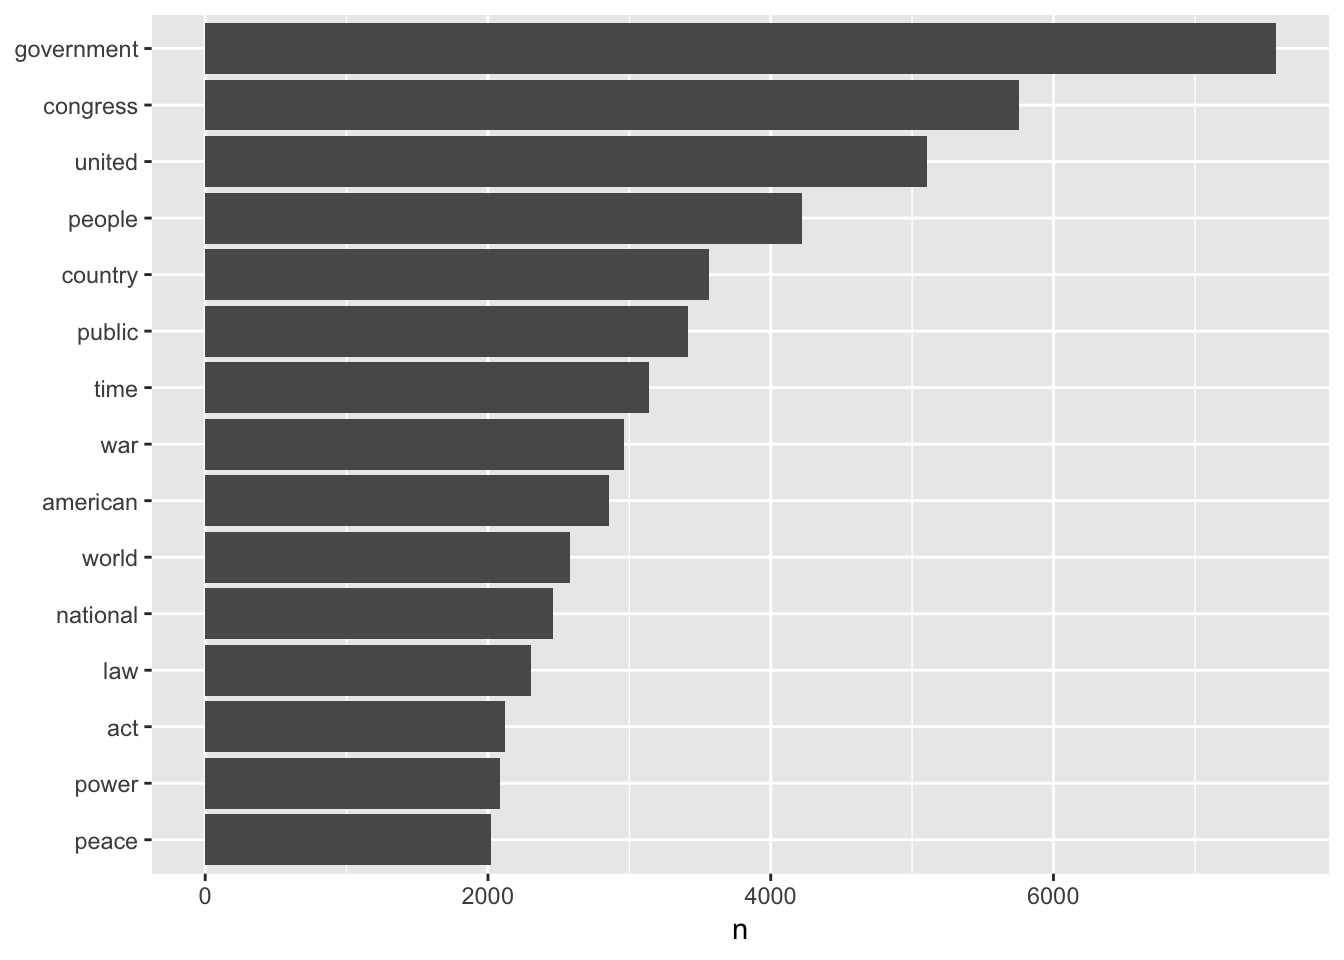
\includegraphics{R-text-analysis_files/figure-latex/unnamed-chunk-14-1.pdf}

What if we're interested in most used words per speech?

\begin{Shaded}
\begin{Highlighting}[]
\CommentTok{# Count words by book}
\NormalTok{doc_words <-}\StringTok{ }\NormalTok{tidy_sotu_words }\OperatorTok
\StringTok{  }\KeywordTok{count}\NormalTok{(doc_id, word, }\DataTypeTok{sort =} \OtherTok{TRUE}\NormalTok{)}

\CommentTok{# Calculate the total number of words by book and save them to a tibble}
\NormalTok{total_words <-}\StringTok{ }\NormalTok{doc_words }\OperatorTok
\StringTok{  }\KeywordTok{group_by}\NormalTok{(doc_id) }\OperatorTok
\StringTok{  }\KeywordTok{summarize}\NormalTok{(}\DataTypeTok{total =} \KeywordTok{sum}\NormalTok{(n))}

\CommentTok{# Join the total column with the rest of the data so we can calculate frequency}
\NormalTok{doc_words <-}\StringTok{ }\KeywordTok{left_join}\NormalTok{(doc_words, total_words)}

\NormalTok{doc_words }
\end{Highlighting}
\end{Shaded}

\begin{verbatim}
#> # A tibble: 352,846 x 4
#>    doc_id                       word               n total
#>    <chr>                        <chr>          <int> <int>
#>  1 harry-s-truman-1946.txt      dollars          207 12614
#>  2 jimmy-carter-1980b.txt       congress         204 16128
#>  3 harry-s-truman-1946.txt      war              201 12614
#>  4 william-howard-taft-1910.txt government       164 11178
#>  5 james-k-polk-1846.txt        mexico           158  7023
#>  6 richard-m-nixon-1974b.txt    federal          141  9996
#>  7 harry-s-truman-1946.txt      million          138 12614
#>  8 harry-s-truman-1946.txt      fiscal           129 12614
#>  9 jimmy-carter-1981.txt        administration   129 16595
#> 10 william-howard-taft-1912.txt government       129 10215
#> # ... with 352,836 more rows
\end{verbatim}

Let's graph the top words per book.

\begin{Shaded}
\begin{Highlighting}[]
\NormalTok{doc_words }\OperatorTok\StringTok{ }
\StringTok{  }\KeywordTok{filter}\NormalTok{(n }\OperatorTok{>}\StringTok{ }\DecValTok{100}\NormalTok{) }\OperatorTok
\StringTok{  }\KeywordTok{ggplot}\NormalTok{(}\KeywordTok{aes}\NormalTok{(word, n, }\DataTypeTok{fill =}\NormalTok{ doc_id)) }\OperatorTok{+}
\StringTok{  }\KeywordTok{geom_col}\NormalTok{() }\OperatorTok{+}\StringTok{ }
\StringTok{  }\KeywordTok{xlab}\NormalTok{(}\OtherTok{NULL}\NormalTok{) }\OperatorTok{+}
\StringTok{  }\KeywordTok{coord_flip}\NormalTok{()}
\end{Highlighting}
\end{Shaded}

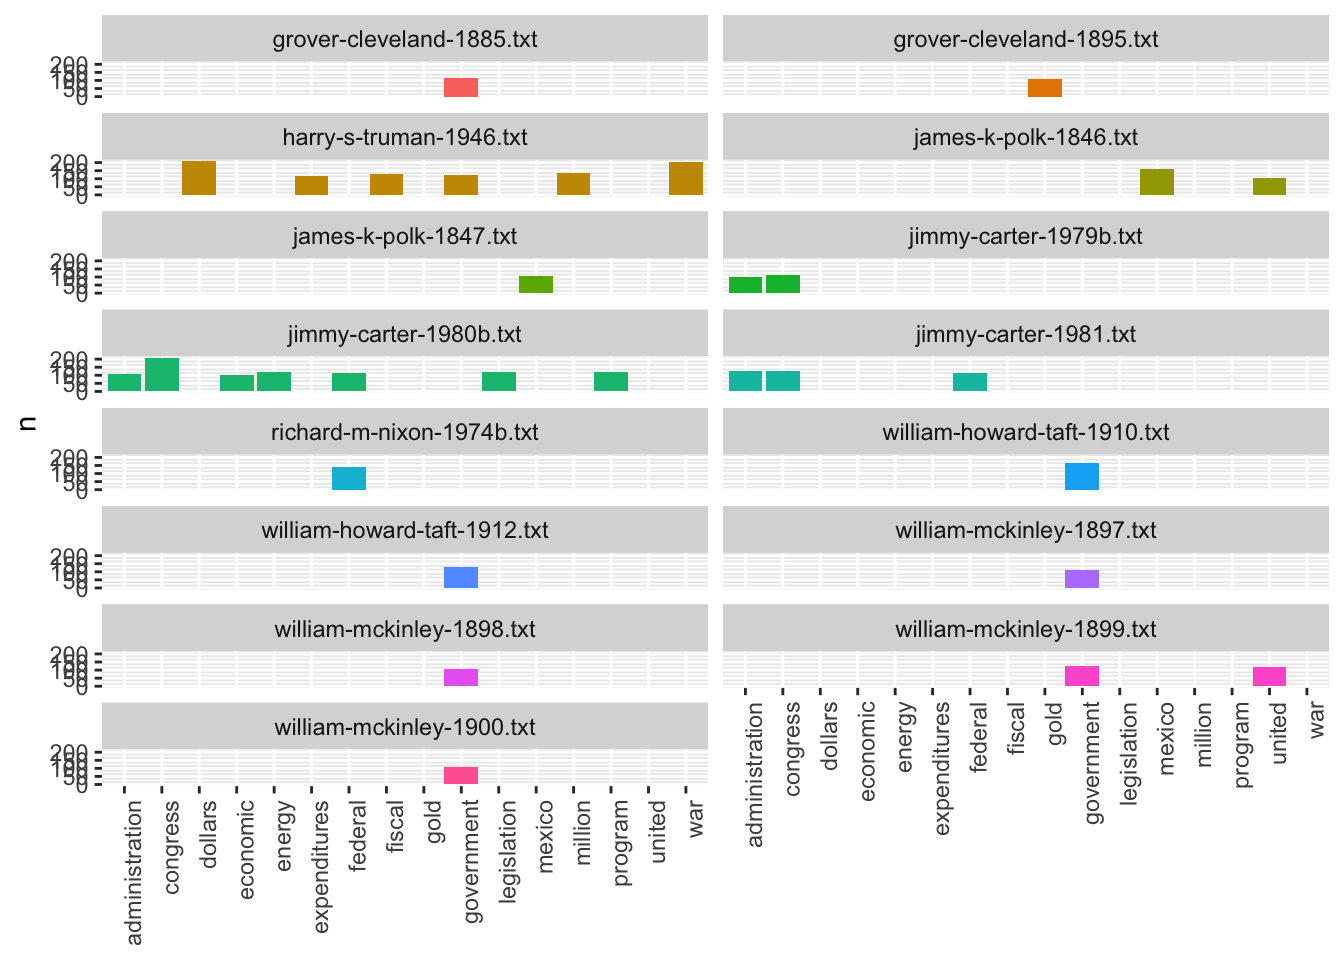
\includegraphics{R-text-analysis_files/figure-latex/unnamed-chunk-16-1.pdf}

That's cool looking, but let's split it into facets so we can see by speech.

\begin{Shaded}
\begin{Highlighting}[]
\NormalTok{doc_words }\OperatorTok\StringTok{ }
\StringTok{  }\KeywordTok{filter}\NormalTok{(n }\OperatorTok{>}\StringTok{ }\DecValTok{100}\NormalTok{) }\OperatorTok
\StringTok{  }\KeywordTok{ggplot}\NormalTok{(}\KeywordTok{aes}\NormalTok{(word, n, }\DataTypeTok{fill =}\NormalTok{ doc_id)) }\OperatorTok{+}
\StringTok{  }\KeywordTok{geom_col}\NormalTok{(}\DataTypeTok{show.legend =} \OtherTok{FALSE}\NormalTok{) }\OperatorTok{+}\StringTok{ }
\StringTok{  }\KeywordTok{xlab}\NormalTok{(}\OtherTok{NULL}\NormalTok{) }\OperatorTok{+}
\StringTok{  }\KeywordTok{facet_wrap}\NormalTok{(}\OperatorTok{~}\NormalTok{doc_id, }\DataTypeTok{ncol =} \DecValTok{2}\NormalTok{) }\OperatorTok{+}\StringTok{ }
\StringTok{  }\KeywordTok{theme}\NormalTok{(}\DataTypeTok{axis.text.x =} \KeywordTok{element_text}\NormalTok{(}\DataTypeTok{angle =} \DecValTok{90}\NormalTok{, }\DataTypeTok{hjust =} \DecValTok{1}\NormalTok{))}
\end{Highlighting}
\end{Shaded}

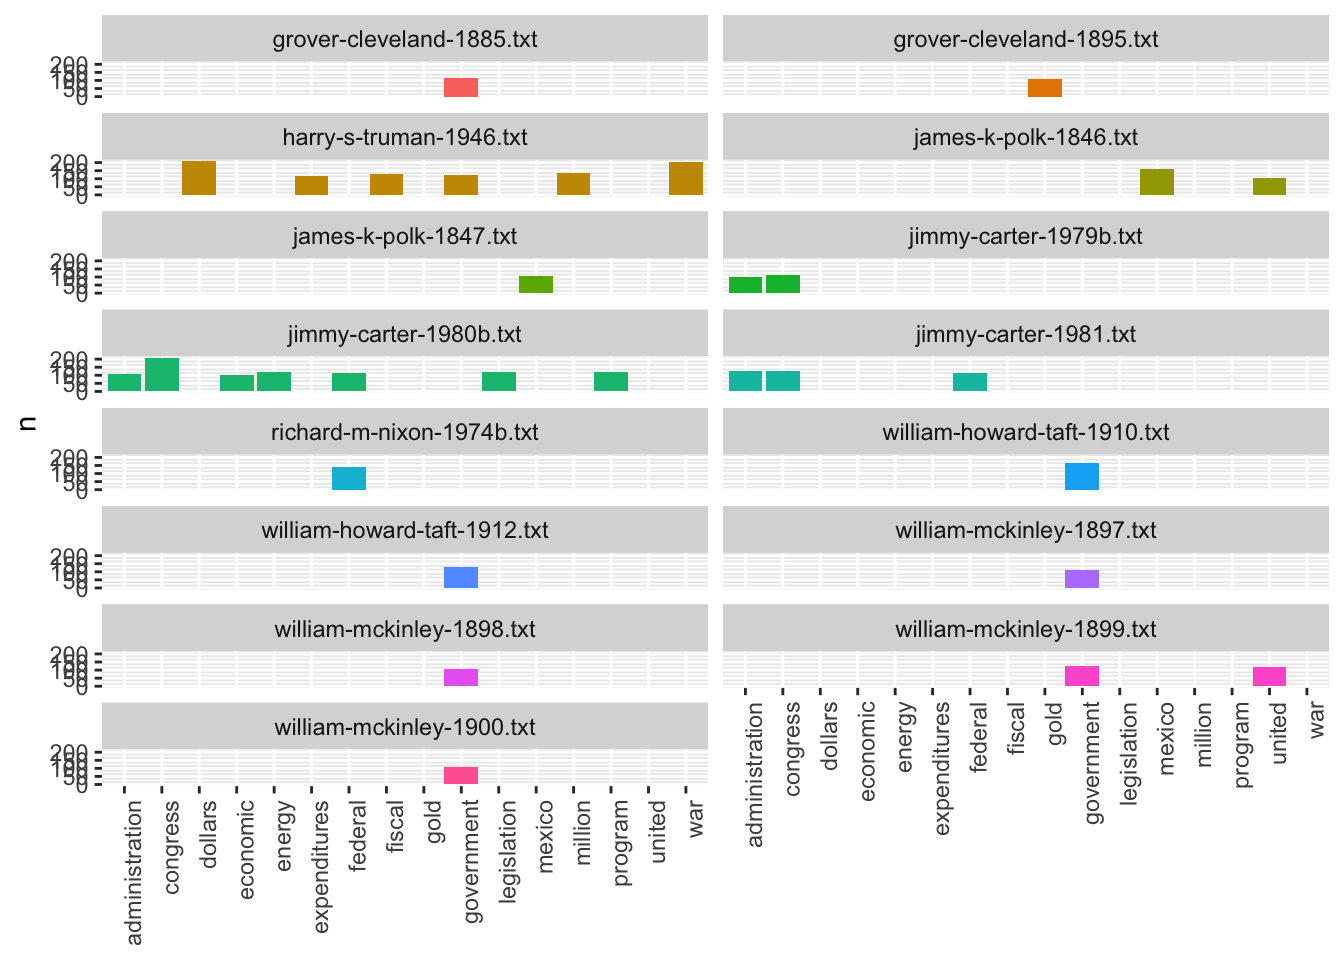
\includegraphics{R-text-analysis_files/figure-latex/unnamed-chunk-17-1.pdf}

We could keep cleaning this figure up by setting some minimum sizing, determining the spacing between y-axis labels better, and so forth, but for now we'll accept it as showing some sense of variation across speeches where certain words are used most.

What if we want to check the most common words per speech for a single president? We could filter this \texttt{doc\_words} dataset based on the president's name being in the doc\_id, but I think it's easier to filter from the initial tidy data and recount.

\begin{Shaded}
\begin{Highlighting}[]
\NormalTok{tidy_sotu_words }\OperatorTok
\StringTok{  }\KeywordTok{filter}\NormalTok{(president }\OperatorTok{==}\StringTok{ "Barack Obama"}\NormalTok{) }\OperatorTok
\StringTok{  }\KeywordTok{count}\NormalTok{(doc_id, word, }\DataTypeTok{sort =} \OtherTok{TRUE}\NormalTok{) }\OperatorTok
\StringTok{  }\KeywordTok{filter}\NormalTok{(n }\OperatorTok{>}\StringTok{ }\DecValTok{20}\NormalTok{) }\OperatorTok
\StringTok{  }\KeywordTok{ggplot}\NormalTok{(}\KeywordTok{aes}\NormalTok{(word, n, }\DataTypeTok{fill=}\NormalTok{doc_id)) }\OperatorTok{+}
\StringTok{  }\KeywordTok{geom_col}\NormalTok{() }\OperatorTok{+}
\StringTok{  }\KeywordTok{facet_wrap}\NormalTok{(}\OperatorTok{~}\NormalTok{doc_id, }\DataTypeTok{ncol =} \DecValTok{2}\NormalTok{) }\OperatorTok{+}\StringTok{ }
\StringTok{  }\KeywordTok{theme}\NormalTok{(}\DataTypeTok{axis.text.x =} \KeywordTok{element_text}\NormalTok{(}\DataTypeTok{angle =} \DecValTok{90}\NormalTok{, }\DataTypeTok{hjust =} \DecValTok{1}\NormalTok{))}
\end{Highlighting}
\end{Shaded}

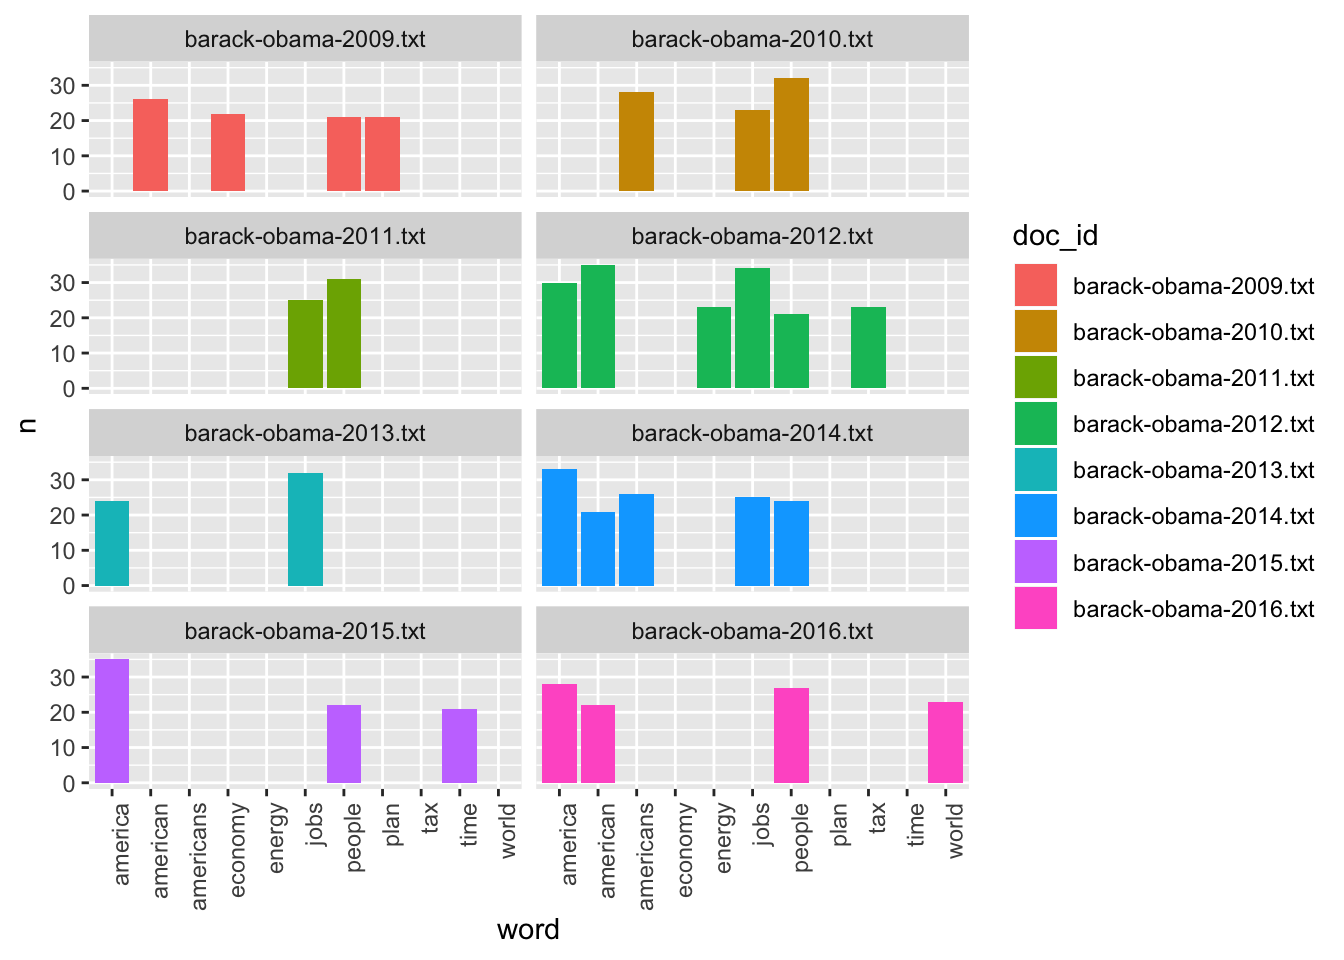
\includegraphics{R-text-analysis_files/figure-latex/unnamed-chunk-18-1.pdf}

\hypertarget{term-frequency}{%
\section{Term frequency}\label{term-frequency}}

Sometimes, a raw count of a word is less important than understanding how often that word appears in respect to the total number of words in a text. This ratio would be the \textbf{term frequency}.

\begin{Shaded}
\begin{Highlighting}[]
\NormalTok{doc_words <-}\StringTok{ }\NormalTok{doc_words }\OperatorTok
\StringTok{  }\KeywordTok{mutate}\NormalTok{(}\DataTypeTok{term_freq =}\NormalTok{ n }\OperatorTok{/}\StringTok{ }\NormalTok{total)}

\NormalTok{doc_words }
\end{Highlighting}
\end{Shaded}

\begin{verbatim}
#> # A tibble: 352,846 x 5
#>    doc_id                       word               n total term_freq
#>    <chr>                        <chr>          <int> <int>     <dbl>
#>  1 harry-s-truman-1946.txt      dollars          207 12614   0.0164 
#>  2 jimmy-carter-1980b.txt       congress         204 16128   0.0126 
#>  3 harry-s-truman-1946.txt      war              201 12614   0.0159 
#>  4 william-howard-taft-1910.txt government       164 11178   0.0147 
#>  5 james-k-polk-1846.txt        mexico           158  7023   0.0225 
#>  6 richard-m-nixon-1974b.txt    federal          141  9996   0.0141 
#>  7 harry-s-truman-1946.txt      million          138 12614   0.0109 
#>  8 harry-s-truman-1946.txt      fiscal           129 12614   0.0102 
#>  9 jimmy-carter-1981.txt        administration   129 16595   0.00777
#> 10 william-howard-taft-1912.txt government       129 10215   0.0126 
#> # ... with 352,836 more rows
\end{verbatim}

Let's graph the term frequency for one of these speeches so we can understand the frequency distribution of words over a text.

\begin{Shaded}
\begin{Highlighting}[]
\NormalTok{doc_words }\OperatorTok
\StringTok{  }\KeywordTok{filter}\NormalTok{(doc_id }\OperatorTok{==}\StringTok{ "harry-s-truman-1946.txt"}\NormalTok{) }\OperatorTok
\StringTok{  }\KeywordTok{ggplot}\NormalTok{(}\KeywordTok{aes}\NormalTok{(term_freq)) }\OperatorTok{+}
\StringTok{  }\KeywordTok{geom_histogram}\NormalTok{(}\DataTypeTok{show.legend =} \OtherTok{FALSE}\NormalTok{) }\OperatorTok{+}
\StringTok{  }\KeywordTok{xlim}\NormalTok{(}\OtherTok{NA}\NormalTok{, }\FloatTok{.012}\NormalTok{)}
\end{Highlighting}
\end{Shaded}

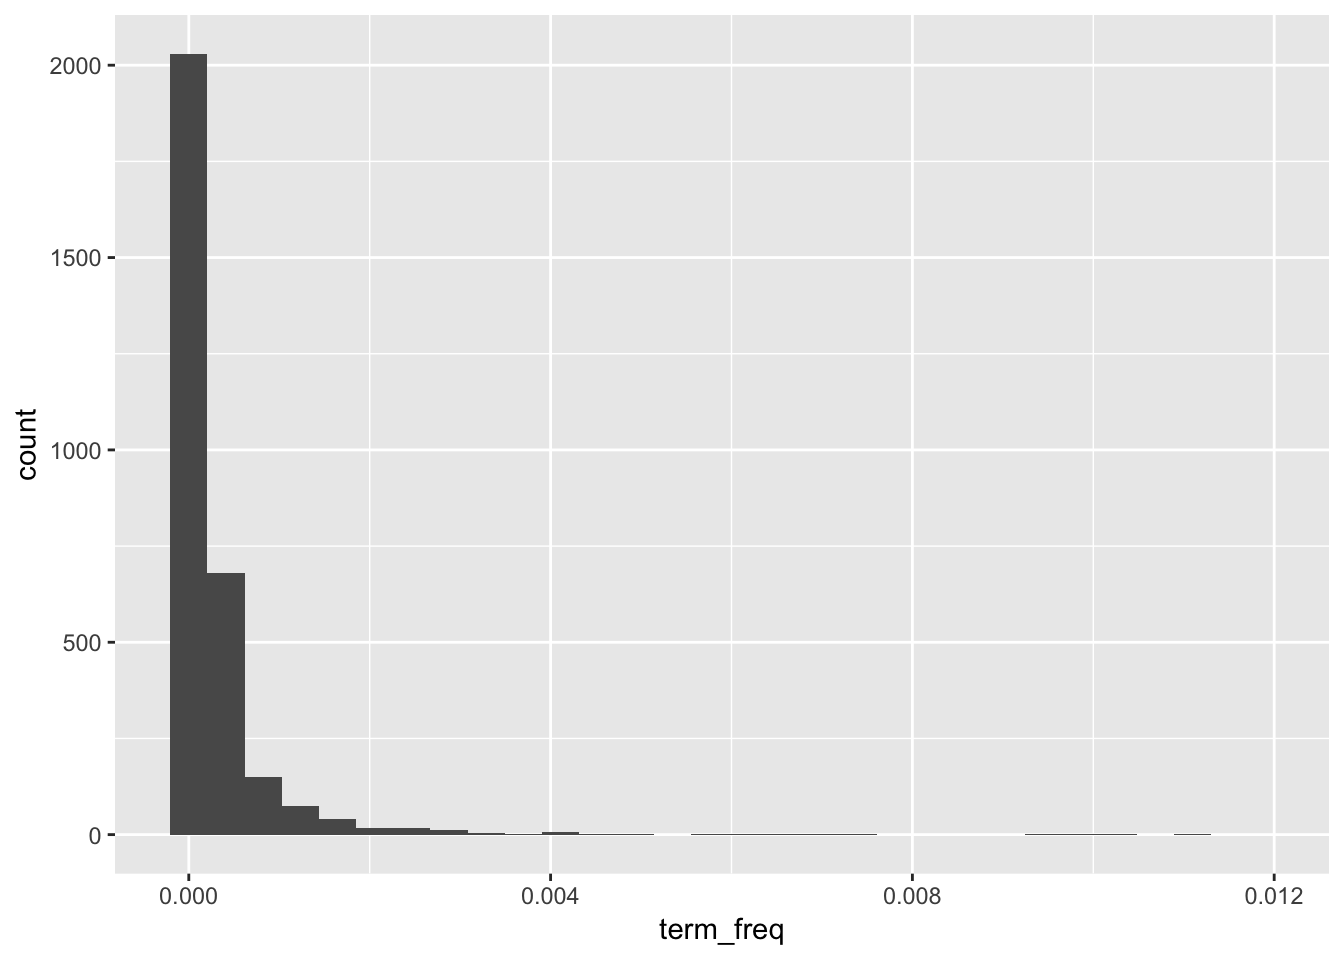
\includegraphics{R-text-analysis_files/figure-latex/unnamed-chunk-20-1.pdf}

This distribution makes sense. Most words are used relatively rarely in a text. Only a few have a high term frequency.

We could keep filtering this data to see which terms have high frequency, thus maybe increased significance, for different presidents and different particular speeches. We could also subset based on decade, and get a sense of what was important in each decade. We're going to take a slightly different approach though. We've been looking at term frequency per document. What if we want to know about words that seem more important based on the contents of the entire corpus?

\hypertarget{tf-idf}{%
\section{Tf-idf}\label{tf-idf}}

For this, we can use term-frequency according to inverse document frequency (tf-idf). Tf-idf measures how important a word is within a corpus by scaling term frequency per document according to the inverse of the term's document frequency (number of documents within the corpus in which the term appears divided by the number of documents).

We could write our own function for tf-idf, but in this case we'll take advantage of tidytext's implementation.

\begin{Shaded}
\begin{Highlighting}[]
\NormalTok{doc_words <-}\StringTok{ }\NormalTok{doc_words }\OperatorTok
\StringTok{  }\KeywordTok{bind_tf_idf}\NormalTok{(word, doc_id, n)}

\NormalTok{doc_words}
\end{Highlighting}
\end{Shaded}

\begin{verbatim}
#> # A tibble: 352,846 x 8
#>    doc_id           word          n total term_freq      tf     idf  tf_idf
#>    <chr>            <chr>     <int> <int>     <dbl>   <dbl>   <dbl>   <dbl>
#>  1 harry-s-truman-~ dollars     207 12614   0.0164  0.0164  0.612   1.00e-2
#>  2 jimmy-carter-19~ congress    204 16128   0.0126  0.0126  0.00425 5.37e-5
#>  3 harry-s-truman-~ war         201 12614   0.0159  0.0159  0.0345  5.50e-4
#>  4 william-howard-~ governme~   164 11178   0.0147  0.0147  0.00425 6.23e-5
#>  5 james-k-polk-18~ mexico      158  7023   0.0225  0.0225  0.810   1.82e-2
#>  6 richard-m-nixon~ federal     141  9996   0.0141  0.0141  0.293   4.14e-3
#>  7 harry-s-truman-~ million     138 12614   0.0109  0.0109  0.728   7.96e-3
#>  8 harry-s-truman-~ fiscal      129 12614   0.0102  0.0102  0.494   5.05e-3
#>  9 jimmy-carter-19~ administ~   129 16595   0.00777 0.00777 0.282   2.19e-3
#> 10 william-howard-~ governme~   129 10215   0.0126  0.0126  0.00425 5.36e-5
#> # ... with 352,836 more rows
\end{verbatim}

The tf-idf value will be:

\begin{itemize}
\tightlist
\item
  lower for words that appear in many documents in the corpus, and lowest when the word occurs in virtually all documents.
\item
  high for words that appear many times in few documents in the corpus, this lending high discriminatory power to those documents.
\end{itemize}

Let's look at some of the words in the corpus that have the highest tf-idf scores, which means words that are particularly distinctive for their documents.

\begin{Shaded}
\begin{Highlighting}[]
\NormalTok{doc_words }\OperatorTok
\StringTok{  }\KeywordTok{select}\NormalTok{(}\OperatorTok{-}\NormalTok{total) }\OperatorTok
\StringTok{  }\KeywordTok{arrange}\NormalTok{(}\KeywordTok{desc}\NormalTok{(tf_idf))}
\end{Highlighting}
\end{Shaded}

\begin{verbatim}
#> # A tibble: 352,846 x 7
#>    doc_id                     word         n term_freq      tf   idf tf_idf
#>    <chr>                      <chr>    <int>     <dbl>   <dbl> <dbl>  <dbl>
#>  1 lyndon-b-johnson-1966.txt  vietnam     32   0.0152  0.0152   2.42 0.0367
#>  2 jimmy-carter-1980a.txt     soviet      31   0.0218  0.0218   1.47 0.0321
#>  3 george-w-bush-2003.txt     hussein     19   0.00811 0.00811  3.85 0.0313
#>  4 george-w-bush-2003.txt     saddam      19   0.00811 0.00811  3.67 0.0298
#>  5 franklin-d-roosevelt-1943~ 1942        13   0.00758 0.00758  3.85 0.0292
#>  6 dwight-d-eisenhower-1961.~ 1953        23   0.00747 0.00747  3.85 0.0288
#>  7 john-adams-1800.txt        gentlem~     8   0.0153  0.0153   1.80 0.0275
#>  8 benjamin-harrison-1892.txt 1892        40   0.00741 0.00741  3.52 0.0261
#>  9 franklin-d-roosevelt-1942~ hitler       7   0.00527 0.00527  4.77 0.0251
#> 10 herbert-hoover-1930.txt    1928        14   0.00711 0.00711  3.52 0.0250
#> # ... with 352,836 more rows
\end{verbatim}

These results seem appropriate given our history. To understand the occurrence of the years we might need to look more closely at the speeches themselves, and determine whether the years are significant or whether they need to be removed from the text. It might be that even if they don't need to be removed from the text overall, they still need to be filtered out within the context of this analysis.

In the same way that we narrowed our analysis to Obama speeches earlier, we could subset the corpus before we calculate the tf-idf score to understand which words are most important for a single president within their sotu speeches. Let's do that for Obama.

\begin{Shaded}
\begin{Highlighting}[]
\NormalTok{obama_tf_idf <-}\StringTok{ }\NormalTok{tidy_sotu_words }\OperatorTok
\StringTok{  }\KeywordTok{filter}\NormalTok{(president }\OperatorTok{==}\StringTok{ "Barack Obama"}\NormalTok{) }\OperatorTok
\StringTok{  }\KeywordTok{count}\NormalTok{(doc_id, word, }\DataTypeTok{sort =} \OtherTok{TRUE}\NormalTok{) }\OperatorTok
\StringTok{  }\KeywordTok{bind_tf_idf}\NormalTok{(word, doc_id, n) }\OperatorTok
\StringTok{  }\KeywordTok{arrange}\NormalTok{(}\KeywordTok{desc}\NormalTok{(tf_idf))}

\NormalTok{obama_tf_idf}
\end{Highlighting}
\end{Shaded}

\begin{verbatim}
#> # A tibble: 10,656 x 6
#>    doc_id                word          n      tf   idf  tf_idf
#>    <chr>                 <chr>     <int>   <dbl> <dbl>   <dbl>
#>  1 barack-obama-2016.txt voices        8 0.00372  2.08 0.00773
#>  2 barack-obama-2014.txt cory          9 0.00322  2.08 0.00671
#>  3 barack-obama-2015.txt rebekah       7 0.00273  2.08 0.00567
#>  4 barack-obama-2012.txt unit          7 0.00255  2.08 0.00531
#>  5 barack-obama-2016.txt isil          8 0.00372  1.39 0.00515
#>  6 barack-obama-2009.txt restart       5 0.00221  2.08 0.00460
#>  7 barack-obama-2013.txt reduction     6 0.00220  2.08 0.00458
#>  8 barack-obama-2015.txt childcare     8 0.00312  1.39 0.00432
#>  9 barack-obama-2011.txt brandon       5 0.00197  2.08 0.00409
#> 10 barack-obama-2015.txt economics     5 0.00195  2.08 0.00405
#> # ... with 10,646 more rows
\end{verbatim}

Based on what you know of the Obama years and sotu speeches generally, how would you interpret these results?

Let's try graphing these results, showing the top tf-idf terms per speech for Obama's speeches.

\begin{Shaded}
\begin{Highlighting}[]
\NormalTok{obama_tf_idf }\OperatorTok
\StringTok{  }\KeywordTok{group_by}\NormalTok{(doc_id) }\OperatorTok
\StringTok{  }\KeywordTok{mutate}\NormalTok{(}\DataTypeTok{word =} \KeywordTok{factor}\NormalTok{(word, }\DataTypeTok{levels =} \KeywordTok{rev}\NormalTok{(}\KeywordTok{unique}\NormalTok{(word)))) }\OperatorTok\StringTok{ }
\StringTok{  }\KeywordTok{group_by}\NormalTok{(doc_id) }\OperatorTok\StringTok{ }
\StringTok{  }\KeywordTok{top_n}\NormalTok{(}\DecValTok{5}\NormalTok{) }\OperatorTok\StringTok{ }
\StringTok{  }\KeywordTok{ungroup}\NormalTok{() }\OperatorTok
\StringTok{  }\KeywordTok{ggplot}\NormalTok{(}\KeywordTok{aes}\NormalTok{(word, tf_idf, }\DataTypeTok{fill =}\NormalTok{ doc_id)) }\OperatorTok{+}
\StringTok{  }\KeywordTok{geom_col}\NormalTok{(}\DataTypeTok{show.legend =} \OtherTok{FALSE}\NormalTok{) }\OperatorTok{+}
\StringTok{  }\KeywordTok{labs}\NormalTok{(}\DataTypeTok{x =} \OtherTok{NULL}\NormalTok{, }\DataTypeTok{y =} \StringTok{"tf-idf"}\NormalTok{) }\OperatorTok{+}
\StringTok{  }\KeywordTok{facet_wrap}\NormalTok{(}\OperatorTok{~}\NormalTok{doc_id, }\DataTypeTok{ncol =} \DecValTok{2}\NormalTok{, }\DataTypeTok{scales =} \StringTok{"free"}\NormalTok{) }\OperatorTok{+}
\StringTok{  }\KeywordTok{coord_flip}\NormalTok{() }\OperatorTok{+}\StringTok{ }
\StringTok{  }\KeywordTok{theme}\NormalTok{(}\DataTypeTok{axis.text.y =} \KeywordTok{element_text}\NormalTok{(}\DataTypeTok{angle =} \DecValTok{45}\NormalTok{)) }
\end{Highlighting}
\end{Shaded}

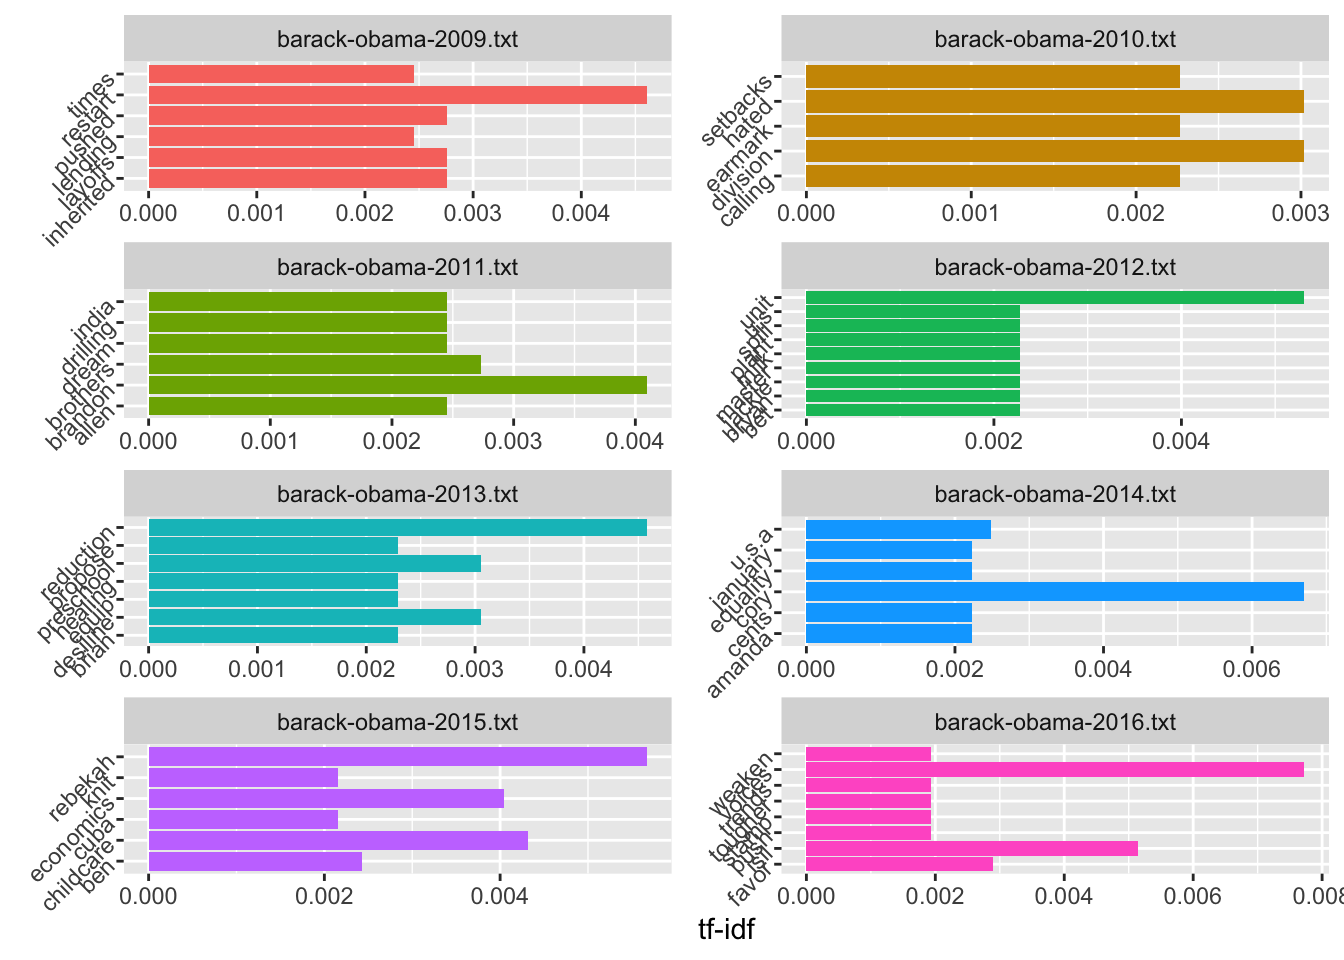
\includegraphics{R-text-analysis_files/figure-latex/unnamed-chunk-24-1.pdf}

\hypertarget{n-grams}{%
\section{N-Grams}\label{n-grams}}

We mentioned n-grams in the intro, but let's revisit them here and take a look at the most common bigrams in the speeches. Remember this is what we get back:

\begin{Shaded}
\begin{Highlighting}[]
\NormalTok{sotu_whole }\OperatorTok
\StringTok{  }\KeywordTok{unnest_tokens}\NormalTok{(bigram, text, }\DataTypeTok{token =} \StringTok{"ngrams"}\NormalTok{, }\DataTypeTok{n =} \DecValTok{2}\NormalTok{) }\CommentTok{# create bigram}
\end{Highlighting}
\end{Shaded}

\begin{verbatim}
#> # A tibble: 1,964,976 x 7
#>    president     year years_active party  sotu_type doc_id       bigram    
#>    <chr>        <int> <chr>        <chr>  <chr>     <chr>        <chr>     
#>  1 Abraham Lin~  1861 1861-1865    Repub~ written   abraham-lin~ fellow ci~
#>  2 Abraham Lin~  1861 1861-1865    Repub~ written   abraham-lin~ citizens ~
#>  3 Abraham Lin~  1861 1861-1865    Repub~ written   abraham-lin~ of the    
#>  4 Abraham Lin~  1861 1861-1865    Repub~ written   abraham-lin~ the senate
#>  5 Abraham Lin~  1861 1861-1865    Repub~ written   abraham-lin~ senate and
#>  6 Abraham Lin~  1861 1861-1865    Repub~ written   abraham-lin~ and house 
#>  7 Abraham Lin~  1861 1861-1865    Repub~ written   abraham-lin~ house of  
#>  8 Abraham Lin~  1861 1861-1865    Repub~ written   abraham-lin~ of repres~
#>  9 Abraham Lin~  1861 1861-1865    Repub~ written   abraham-lin~ represent~
#> 10 Abraham Lin~  1861 1861-1865    Repub~ written   abraham-lin~ in the    
#> # ... with 1,964,966 more rows
\end{verbatim}

Let's see the most common bigrams:

\begin{Shaded}
\begin{Highlighting}[]
\NormalTok{sotu_whole }\OperatorTok
\StringTok{  }\KeywordTok{unnest_tokens}\NormalTok{(bigram, text, }\DataTypeTok{token =} \StringTok{"ngrams"}\NormalTok{, }\DataTypeTok{n =} \DecValTok{2}\NormalTok{) }\OperatorTok\StringTok{ }
\StringTok{  }\KeywordTok{count}\NormalTok{(bigram, }\DataTypeTok{sort =} \OtherTok{TRUE}\NormalTok{) }\CommentTok{# count ocurrences and sord descending}
\end{Highlighting}
\end{Shaded}

\begin{verbatim}
#> # A tibble: 469,092 x 2
#>    bigram            n
#>    <chr>         <int>
#>  1 of the        33610
#>  2 in the        12499
#>  3 to the        11643
#>  4 for the        6892
#>  5 and the        6224
#>  6 by the         5606
#>  7 of our         5172
#>  8 the united     4767
#>  9 united states  4760
#> 10 it is          4756
#> # ... with 469,082 more rows
\end{verbatim}

Ok, so we again need to remove the stopwords. This time let's use dplyr's \texttt{filter} function for this. And before that we will \texttt{separate} the two words into two columns.

\begin{Shaded}
\begin{Highlighting}[]
\NormalTok{sotu_bigrams <-}\StringTok{ }\NormalTok{sotu_whole }\OperatorTok
\StringTok{  }\KeywordTok{unnest_tokens}\NormalTok{(bigram, text, }\DataTypeTok{token =} \StringTok{"ngrams"}\NormalTok{, }\DataTypeTok{n =} \DecValTok{2}\NormalTok{) }\OperatorTok\StringTok{ }
\StringTok{  }\KeywordTok{separate}\NormalTok{(bigram, }\KeywordTok{c}\NormalTok{(}\StringTok{"word1"}\NormalTok{, }\StringTok{"word2"}\NormalTok{), }\DataTypeTok{sep =} \StringTok{" "}\NormalTok{) }\OperatorTok\StringTok{ }\CommentTok{# separate into cols}
\StringTok{  }\KeywordTok{filter}\NormalTok{(}\OperatorTok{!}\NormalTok{word1 }\OperatorTok\StringTok{ }\NormalTok{stop_words}\OperatorTok{$}\NormalTok{word) }\OperatorTok\StringTok{ }\CommentTok{# remove stopwords}
\StringTok{  }\KeywordTok{filter}\NormalTok{(}\OperatorTok{!}\NormalTok{word2 }\OperatorTok\StringTok{ }\NormalTok{stop_words}\OperatorTok{$}\NormalTok{word)}

\NormalTok{sotu_bigrams }\OperatorTok\StringTok{ }
\StringTok{  }\KeywordTok{count}\NormalTok{(word1, word2, }\DataTypeTok{sort =} \OtherTok{TRUE}\NormalTok{)}
\end{Highlighting}
\end{Shaded}

\begin{verbatim}
#> # A tibble: 129,622 x 3
#>    word1    word2          n
#>    <chr>    <chr>      <int>
#>  1 federal  government   479
#>  2 american people       428
#>  3 june     30           325
#>  4 fellow   citizens     296
#>  5 public   debt         283
#>  6 public   lands        256
#>  7 health   care         240
#>  8 social   security     232
#>  9 post     office       202
#> 10 annual   message      200
#> # ... with 129,612 more rows
\end{verbatim}

(Bonus question: What happened on that June 30th?)

A bigram can also be treated as a term in a document in the same way that we treated individual words. That means we can look at tf-idf values in the same way.

First we will re-unite the two word columns again, and then generate the tf-idf count as above.

\begin{Shaded}
\begin{Highlighting}[]
\NormalTok{bigram_tf_idf <-}\StringTok{ }\NormalTok{sotu_bigrams }\OperatorTok
\StringTok{  }\KeywordTok{unite}\NormalTok{(bigram, word1, word2, }\DataTypeTok{sep =} \StringTok{" "}\NormalTok{) }\OperatorTok\StringTok{ }\CommentTok{# combine columns}
\StringTok{  }\KeywordTok{count}\NormalTok{(president, bigram) }\OperatorTok
\StringTok{  }\KeywordTok{bind_tf_idf}\NormalTok{(bigram, president, n) }\OperatorTok
\StringTok{  }\KeywordTok{arrange}\NormalTok{(}\KeywordTok{desc}\NormalTok{(tf_idf))}
\end{Highlighting}
\end{Shaded}

What makes the speeches of different presidents unique?

Let's pick a few presidents and plot their highest scoring tf-idf values here.

\begin{Shaded}
\begin{Highlighting}[]
\NormalTok{potus <-}\StringTok{ }\KeywordTok{c}\NormalTok{(}\StringTok{"John F. Kennedy"}\NormalTok{, }\StringTok{"Richard M. Nixon"}\NormalTok{, }\StringTok{"George Bush"}\NormalTok{, }\StringTok{"George W. Bush"}\NormalTok{)}

\NormalTok{bigram_tf_idf }\OperatorTok
\StringTok{  }\KeywordTok{filter}\NormalTok{(president }\OperatorTok\StringTok{ }\NormalTok{potus) }\OperatorTok\StringTok{ }
\StringTok{  }\KeywordTok{group_by}\NormalTok{(president) }\OperatorTok\StringTok{ }
\StringTok{  }\KeywordTok{top_n}\NormalTok{(}\DecValTok{20}\NormalTok{) }\OperatorTok\StringTok{ }
\StringTok{  }\KeywordTok{ggplot}\NormalTok{(}\KeywordTok{aes}\NormalTok{(}\KeywordTok{reorder}\NormalTok{(bigram, tf_idf), tf_idf, }\DataTypeTok{fill =}\NormalTok{ president)) }\OperatorTok{+}
\StringTok{  }\KeywordTok{geom_col}\NormalTok{(}\DataTypeTok{show.legend =} \OtherTok{FALSE}\NormalTok{) }\OperatorTok{+}
\StringTok{  }\KeywordTok{labs}\NormalTok{(}\DataTypeTok{x =} \OtherTok{NULL}\NormalTok{, }\DataTypeTok{y =} \StringTok{"tf-idf"}\NormalTok{) }\OperatorTok{+}
\StringTok{  }\KeywordTok{facet_wrap}\NormalTok{(}\OperatorTok{~}\NormalTok{president, }\DataTypeTok{scales =} \StringTok{"free"}\NormalTok{, }\DataTypeTok{nrow =} \DecValTok{2}\NormalTok{) }\OperatorTok{+}
\StringTok{  }\KeywordTok{coord_flip}\NormalTok{()}
\end{Highlighting}
\end{Shaded}

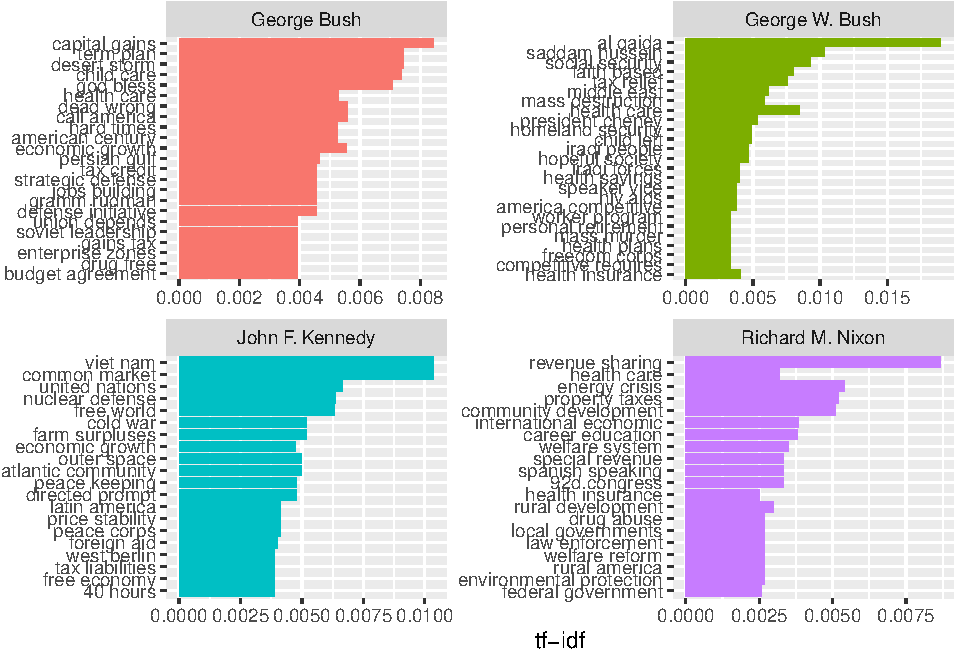
\includegraphics{R-text-analysis_files/figure-latex/bigram-tf-idf-plot-1.pdf}

\hypertarget{co-occurrence}{%
\section{Co-occurrence}\label{co-occurrence}}

Co-occurrences give us a sense of words that appear in the same text, but not necessarily next to each other.

For this section we will make use of the \texttt{widyr} package. It allows us to turn our table into a wide matrix. In our case that matrix will be made up of the individual words and the cell values will be the counts of how many times they co-occur. Then we will turn the matrix back into a tidy form, where each row contains the word pairs and the count of their co-occurrence. This lets us count common pairs of words co-appearing within the same speech.

The function which helps us do this is the \texttt{pairwise\_count()} function.

Since processing the entire corpus would take too long here, we will only look at the last 20 words of each speech.

\begin{Shaded}
\begin{Highlighting}[]
\KeywordTok{library}\NormalTok{(widyr)}

\CommentTok{# extract last 100 words from text}
\NormalTok{sotu_whole}\OperatorTok{$}\NormalTok{speech_end <-}\StringTok{ }\KeywordTok{word}\NormalTok{(sotu_whole}\OperatorTok{$}\NormalTok{text, }\DecValTok{-100}\NormalTok{, }\DataTypeTok{end =} \DecValTok{-1}\NormalTok{)}

\NormalTok{sotu_word_pairs <-}\StringTok{ }\NormalTok{sotu_whole }\OperatorTok\StringTok{ }
\StringTok{  }\KeywordTok{unnest_tokens}\NormalTok{(word, speech_end) }\OperatorTok\StringTok{ }
\StringTok{  }\KeywordTok{filter}\NormalTok{(}\OperatorTok{!}\NormalTok{word }\OperatorTok\StringTok{ }\NormalTok{stop_words}\OperatorTok{$}\NormalTok{word) }\OperatorTok\StringTok{ }\CommentTok{# remove stopwords}
\StringTok{  }\KeywordTok{pairwise_count}\NormalTok{(word, doc_id, }\DataTypeTok{sort =} \OtherTok{TRUE}\NormalTok{, }\DataTypeTok{upper =} \OtherTok{FALSE}\NormalTok{) }\CommentTok{# don't include upper triangle of matrix}

\NormalTok{sotu_word_pairs}
\end{Highlighting}
\end{Shaded}

\begin{verbatim}
#> # A tibble: 125,576 x 3
#>    item1      item2       n
#>    <chr>      <chr>   <dbl>
#>  1 god        bless      37
#>  2 god        america    35
#>  3 bless      america    30
#>  4 people     country    26
#>  5 world      god        22
#>  6 god        people     22
#>  7 government people     21
#>  8 congress   people     21
#>  9 public     country    21
#> 10 god        nation     21
#> # ... with 125,566 more rows
\end{verbatim}

To plot the co-occurrence network, we use the \texttt{igraph} library to convert our table into a network graph and \texttt{ggraph} which adds functionality to ggplot and makes it easier to create a network plot.

\begin{Shaded}
\begin{Highlighting}[]
\KeywordTok{library}\NormalTok{(igraph)}
\KeywordTok{library}\NormalTok{(ggraph)}

\NormalTok{sotu_word_pairs }\OperatorTok\StringTok{ }
\StringTok{  }\KeywordTok{filter}\NormalTok{(n }\OperatorTok{>=}\StringTok{ }\DecValTok{10}\NormalTok{) }\OperatorTok\StringTok{  }\CommentTok{# only word pairs that occur 10 or more times}
\StringTok{  }\KeywordTok{graph_from_data_frame}\NormalTok{() }\OperatorTok\StringTok{ }\CommentTok{#convert to graph}
\StringTok{  }\KeywordTok{ggraph}\NormalTok{(}\DataTypeTok{layout =} \StringTok{"fr"}\NormalTok{) }\OperatorTok{+}\StringTok{ }\CommentTok{# place nodes according to the force-directed algorithm of Fruchterman and Reingold}
\StringTok{  }\KeywordTok{geom_edge_link}\NormalTok{(}\KeywordTok{aes}\NormalTok{(}\DataTypeTok{edge_alpha =}\NormalTok{ n, }\DataTypeTok{edge_width =}\NormalTok{ n), }\DataTypeTok{edge_colour =} \StringTok{"tomato"}\NormalTok{) }\OperatorTok{+}
\StringTok{  }\KeywordTok{geom_node_point}\NormalTok{(}\DataTypeTok{size =} \DecValTok{5}\NormalTok{) }\OperatorTok{+}
\StringTok{  }\KeywordTok{geom_node_text}\NormalTok{(}\KeywordTok{aes}\NormalTok{(}\DataTypeTok{label =}\NormalTok{ name), }\DataTypeTok{repel =} \OtherTok{TRUE}\NormalTok{, }
                 \DataTypeTok{point.padding =} \KeywordTok{unit}\NormalTok{(}\FloatTok{0.2}\NormalTok{, }\StringTok{"lines"}\NormalTok{)) }\OperatorTok{+}
\StringTok{  }\KeywordTok{theme_void}\NormalTok{()}
\end{Highlighting}
\end{Shaded}

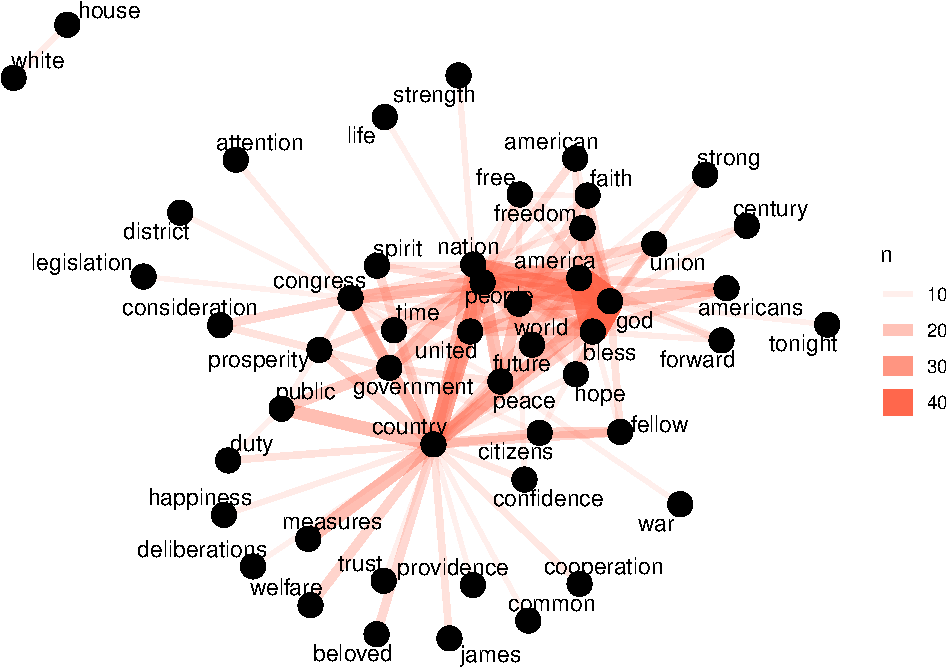
\includegraphics{R-text-analysis_files/figure-latex/plot-network-1.pdf}

There are alternative approaches for this as well. See for example the \texttt{findAssocs} function in the \texttt{tm} package.

\hypertarget{document-term-matrix}{%
\section{Document-Term Matrix}\label{document-term-matrix}}

A \href{https://en.wikipedia.org/wiki/Document-term_matrix}{document-term matrix (DTM)} is a format which is frequently used in text analysis. It is a matrix where we can see the counts of each term per document. In a DTM each row represents a document, each column represents a term, and the cell values are the counts of the occurrences of the term for the particular document.

\texttt{tidytext} provides functionality to convert to and from DTMs, if for example, your analyis requires specific functions that require you to use a different R package which only works with DTM objects.

The \texttt{cast\_dtm} function can be used to create a DTM object from a tidy table.

Let's assume that for some reason we want to use the \texttt{findAssoc} function from the \texttt{tm} package.

First we use dplyr to create a table with the document name, the term, and the count.

\begin{Shaded}
\begin{Highlighting}[]
\CommentTok{# make a table with document, term, count}
\NormalTok{tidy_sotu_words }\OperatorTok\StringTok{ }
\StringTok{  }\KeywordTok{count}\NormalTok{(doc_id, word) }
\end{Highlighting}
\end{Shaded}

\begin{verbatim}
#> # A tibble: 352,846 x 3
#>    doc_id                   word               n
#>    <chr>                    <chr>          <int>
#>  1 abraham-lincoln-1861.txt 1,470,018          1
#>  2 abraham-lincoln-1861.txt 1,500              1
#>  3 abraham-lincoln-1861.txt 100,000            1
#>  4 abraham-lincoln-1861.txt 102,532,509.27     1
#>  5 abraham-lincoln-1861.txt 12,528,000         1
#>  6 abraham-lincoln-1861.txt 13,606,759.11      1
#>  7 abraham-lincoln-1861.txt 1830               1
#>  8 abraham-lincoln-1861.txt 1859               1
#>  9 abraham-lincoln-1861.txt 1860               2
#> 10 abraham-lincoln-1861.txt 1861               6
#> # ... with 352,836 more rows
\end{verbatim}

Now we cast it as a DTM.

\begin{Shaded}
\begin{Highlighting}[]
\NormalTok{sotu_dtm <-}\StringTok{ }\NormalTok{tidy_sotu_words }\OperatorTok\StringTok{ }
\StringTok{  }\KeywordTok{count}\NormalTok{(doc_id, word) }\OperatorTok\StringTok{ }
\StringTok{  }\KeywordTok{cast_dtm}\NormalTok{(doc_id, word, n) }

\KeywordTok{class}\NormalTok{(sotu_dtm)}
\end{Highlighting}
\end{Shaded}

\begin{verbatim}
#> [1] "DocumentTermMatrix"    "simple_triplet_matrix"
\end{verbatim}

Finally, let's use it in the \texttt{tm} package.

\begin{Shaded}
\begin{Highlighting}[]
\KeywordTok{library}\NormalTok{(tm)}

\CommentTok{# look at the terms with tm function}
\KeywordTok{Terms}\NormalTok{(sotu_dtm) }\OperatorTok\StringTok{ }\KeywordTok{tail}\NormalTok{()}
\end{Highlighting}
\end{Shaded}

\begin{verbatim}
#> [1] "queretaro"    "refreshments" "schleswig"    "sedulous"    
#> [5] "subagents"    "transcript"
\end{verbatim}

\begin{Shaded}
\begin{Highlighting}[]
\CommentTok{# most frequent terms}
\KeywordTok{findFreqTerms}\NormalTok{(sotu_dtm, }\DataTypeTok{lowfreq =} \DecValTok{5000}\NormalTok{)}
\end{Highlighting}
\end{Shaded}

\begin{verbatim}
#> [1] "congress"   "government" "united"
\end{verbatim}

\begin{Shaded}
\begin{Highlighting}[]
\CommentTok{# find terms associated with ...}
\KeywordTok{findAssocs}\NormalTok{(sotu_dtm, }\StringTok{"citizen"}\NormalTok{, }\DataTypeTok{corlimit =} \FloatTok{0.5}\NormalTok{)}
\end{Highlighting}
\end{Shaded}

\begin{verbatim}
#> $citizen
#>        laws citizenship  protection   contained    entitled  government 
#>        0.62        0.59        0.56        0.55        0.53        0.53 
#>    citizens  postmaster     careful    question      report       suits 
#>        0.52        0.52        0.51        0.51        0.51        0.51
\end{verbatim}

Conversely, \texttt{tidytext} implements the \texttt{tidy} function (originally from the \texttt{broom} package) to import DocumentTermMatrix objects. Note that it only takes the cells from the DTM that are not 0, so there will be no rows with 0 counts.

\hypertarget{sentiment-analysis}{%
\section{Sentiment analysis}\label{sentiment-analysis}}

\texttt{tidytext} comes with a dataset \texttt{sentiments} which contains several sentiment lexicons, where each word is attributed a certain sentiment, like this:

\begin{Shaded}
\begin{Highlighting}[]
\NormalTok{sentiments}
\end{Highlighting}
\end{Shaded}

\begin{verbatim}
#> # A tibble: 27,314 x 4
#>    word        sentiment lexicon score
#>    <chr>       <chr>     <chr>   <int>
#>  1 abacus      trust     nrc        NA
#>  2 abandon     fear      nrc        NA
#>  3 abandon     negative  nrc        NA
#>  4 abandon     sadness   nrc        NA
#>  5 abandoned   anger     nrc        NA
#>  6 abandoned   fear      nrc        NA
#>  7 abandoned   negative  nrc        NA
#>  8 abandoned   sadness   nrc        NA
#>  9 abandonment anger     nrc        NA
#> 10 abandonment fear      nrc        NA
#> # ... with 27,304 more rows
\end{verbatim}

Here we will take a look at how the sentiment of the speeches change over time. We will use the lexicon from \href{https://www.cs.uic.edu/~liub/FBS/sentiment-analysis.html}{Bing Liu and collaborators}, which assigns positive/negative labels for each word:

\begin{Shaded}
\begin{Highlighting}[]
\NormalTok{bing_lex <-}\StringTok{ }\KeywordTok{get_sentiments}\NormalTok{(}\StringTok{"bing"}\NormalTok{)}
\NormalTok{bing_lex}
\end{Highlighting}
\end{Shaded}

\begin{verbatim}
#> # A tibble: 6,788 x 2
#>    word        sentiment
#>    <chr>       <chr>    
#>  1 2-faced     negative 
#>  2 2-faces     negative 
#>  3 a+          positive 
#>  4 abnormal    negative 
#>  5 abolish     negative 
#>  6 abominable  negative 
#>  7 abominably  negative 
#>  8 abominate   negative 
#>  9 abomination negative 
#> 10 abort       negative 
#> # ... with 6,778 more rows
\end{verbatim}

Since this is a regular tibble, we can use these sentiments and join them to the words of our speeches. We will use \texttt{inner\_join} from \texttt{dplyr}. Since our columns to join on have the same name (\texttt{word}) we don't need to explicitly name it.

\begin{Shaded}
\begin{Highlighting}[]
\NormalTok{tidy_sotu_words }\OperatorTok\StringTok{ }
\StringTok{  }\KeywordTok{inner_join}\NormalTok{(bing_lex) }\OperatorTok\StringTok{ }\CommentTok{# join}
\StringTok{  }\KeywordTok{count}\NormalTok{(year, sentiment) }\CommentTok{# group by year and sentiment}
\end{Highlighting}
\end{Shaded}

\begin{verbatim}
#> # A tibble: 450 x 3
#>     year sentiment     n
#>    <int> <chr>     <int>
#>  1  1790 negative     39
#>  2  1790 positive    125
#>  3  1791 negative     52
#>  4  1791 positive    103
#>  5  1792 negative     57
#>  6  1792 positive     78
#>  7  1793 negative     58
#>  8  1793 positive     72
#>  9  1794 negative    110
#> 10  1794 positive    106
#> # ... with 440 more rows
\end{verbatim}

Finally we can visualize it like this:

\begin{Shaded}
\begin{Highlighting}[]
\NormalTok{tidy_sotu_words }\OperatorTok\StringTok{ }
\StringTok{  }\KeywordTok{inner_join}\NormalTok{(bing_lex) }\OperatorTok\StringTok{ }\CommentTok{# join}
\StringTok{  }\KeywordTok{count}\NormalTok{(year, sentiment) }\OperatorTok\StringTok{ }\CommentTok{# group by year and sentiment}
\StringTok{  }\KeywordTok{ggplot}\NormalTok{(}\KeywordTok{aes}\NormalTok{(year, n, }\DataTypeTok{color =}\NormalTok{ sentiment)) }\OperatorTok{+}
\StringTok{    }\KeywordTok{geom_line}\NormalTok{() }\OperatorTok{+}
\StringTok{    }\KeywordTok{scale_x_continuous}\NormalTok{(}\DataTypeTok{breaks =} \KeywordTok{seq}\NormalTok{(}\DecValTok{1790}\NormalTok{, }\DecValTok{2016}\NormalTok{, }\DataTypeTok{by =} \DecValTok{10}\NormalTok{)) }\OperatorTok{+}
\StringTok{    }\KeywordTok{theme}\NormalTok{(}\DataTypeTok{axis.text.x =} \KeywordTok{element_text}\NormalTok{(}\DataTypeTok{angle =} \DecValTok{45}\NormalTok{, }\DataTypeTok{hjust =} \DecValTok{1}\NormalTok{))}
\end{Highlighting}
\end{Shaded}

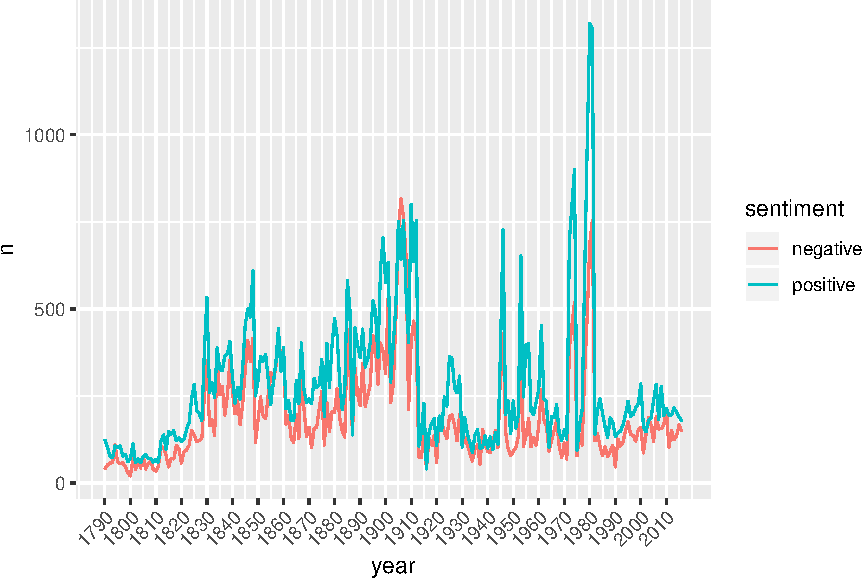
\includegraphics{R-text-analysis_files/figure-latex/sentiment-plot-1.pdf}

\bibliography{book.bib,packages.bib}


\end{document}
